
% !TEX program = xelatex % (can also use "lualatex")
\documentclass[a4paper,11pt,oneside]{book}

% Language
\usepackage[english]{babel}
\usepackage{csquotes}
\usepackage[table]{xcolor}
\usepackage{float}
\definecolor{accentblue}{RGB}{196,215,235}
\definecolor{accentdark}{RGB}{86,118,150}
\usepackage{booktabs}
\usepackage{tabularx}
\usepackage{array}
\usepackage{ragged2e}

\usepackage{xcolor}
\usepackage{tikz}
\usetikzlibrary{positioning,arrows.meta,calc}

\usepackage{pifont}
\newcommand{\cmark}{\ding{51}}
\newcommand{\xmark}{\ding{55}}

% Control design of table of contents
\usepackage{tocloft}

% Blank lines between paragraphs
\usepackage[parfill]{parskip}

% Hyperlinks
\usepackage[hidelinks]{hyperref}

% Extensions of hyperref
\usepackage{bookmark}
\usepackage{nameref}

% Images
\usepackage{graphicx}
\usepackage{pdfpages}
\usepackage{pdflscape}

% Bibliography
\usepackage[
  backend=biber,
  style=apa,
  sortcites=true
]{biblatex}

\DeclareLanguageMapping{english}{english-apa}

\addbibresource{config/literature.bib}
% Page margins
\usepackage{anysize}

% Chapter title formatting
\usepackage{titlesec}

% Remove headers and footers from empty pages
\usepackage{emptypage}

% Glossaries, acronyms, and abbreviations
\usepackage[nopostdot,nogroupskip,toc,acronym,nomain]{glossaries-extra}

% Disable warnings
\usepackage{silence}

% Algorithms and pseudocode
\usepackage{algorithm}
\usepackage[noEnd=true,italicComments=false,commentColor=black]{algpseudocodex}

% Code listings
\usepackage{listings}

% Adjust captions
\usepackage{caption}

% Mathematical alphabets
\usepackage{amssymb}

% Add line breaks to table cells
\usepackage{makecell}

% Header and footer
\usepackage{fancyhdr}

% Appendix
\usepackage{appendix}

% Page Format
\usepackage{fontspec}
\setmainfont{Arial}
\setsansfont{Arial}
\usepackage{setspace}

% LTeX: enabled=false

% Custom column types for tables
\newcolumntype{L}[1]{>{\raggedright\arraybackslash}p{#1}}
\newcolumntype{Y}{>{\raggedright\arraybackslash}X}

% Do not stretch the page contents to the bottom
\raggedbottom

\onehalfspacing
% Reduce hyphenation
\tolerance=500
\emergencystretch=2em
\hyphenpenalty=500
\exhyphenpenalty=500

% Reduce widows and orphans
\widowpenalties=4 10000 10000 500 0
\clubpenalties=4 10000 10000 500 0

% Reduce page breaks in paragraphs
\interlinepenalty=500

% Margins (Left, Right, Top, Bottom)
\marginsize{25mm}{25mm}{25mm}{25mm}

% Chapter title formatting
\titleformat{\chapter}
{\Huge\bfseries}   % format
{\thechapter}      % label
{10pt}             % sep
{}                 % before-code

% Redefine command for vertical centering text in X column (tabularx)
\renewcommand\tabularxcolumn[1]{m{#1}}

% Include chapter number in algorithm numbering.
\renewcommand{\thealgorithm}{\thechapter.\arabic{algorithm}}

% Add double colon after algorithm numbering.
\captionsetup[algorithm]{labelsep=colon}

% Redefine title for list of code listings
\renewcommand{\lstlistlistingname}{List of Code Listings}

% Styling for code listings
\definecolor{stringcolor}{cmyk}{0.8, 0.0, 0.8, 0.2}
\definecolor{commentcolor}{cmyk}{0.0, 0.0, 0.0, 0.5}
\definecolor{emphcolor}{cmyk}{1.0, 0.6, 0.0, 0.2}
\definecolor{keywordcolor}{cmyk}{0.0, 0.5, 1.0, 0.2}

% Define a custom style for listings
\lstdefinestyle{custom_listing_style}{
  language=Python,
  basicstyle=\ttfamily\small,
  columns=fullflexible,
  keepspaces=true,
  frame=tb,
  rulecolor=\color{black},
  numbers=left,
  xleftmargin=2em,
  framexleftmargin=1.5em,
  numberstyle=\scriptsize,
  numbersep=8pt,
  stepnumber=1,
  breaklines=true,
  tabsize=4,
  belowcaptionskip=12pt,
  showstringspaces=false,
  morekeywords={self},
  sensitive=true,
  emph={},
  morestring=[b]",
  morecomment=[l]{//},
  keywordstyle=\color{keywordcolor},
  stringstyle=\color{stringcolor},
  commentstyle=\color{commentcolor},
  emphstyle=\color{emphcolor},
  escapeinside={(*@}{@*)}
}

\lstset{style=custom_listing_style}

% Increase vertical padding for tables
\renewcommand{\arraystretch}{1.5}

% Header and footer
\renewcommand{\chaptermark}[1]{\markboth{#1}{}}

\fancyhf{} % clear all header/footer
\fancyhead[L]{\thechapter\hspace{1.0em}\leftmark}
\fancyfoot[R]{\thepage}

% Make plain style (frontmatter, chapter openings, appendix) match
\fancypagestyle{plain}{%
  \fancyhf{}
  \fancyfoot[R]{\thepage}
  \renewcommand{\headrulewidth}{0pt}
}

% Adjust headheight for header
\setlength{\headheight}{15pt}

% Adjust algpseudocodex keywords
\algrenewcommand\algorithmicrequire{Input:}
\algrenewcommand\algorithmicensure{Output:}

% Definition of custom glossary style for list of abbreviations
\newglossarystyle{customglossarystyle}{
  \setglossarystyle{long}

  % Adjust list of abbreviations to full text width
  \renewenvironment{theglossary}
  {
    \setlength{\tabcolsep}{2pt}%
    \begin{longtable}[l]{@{}p{2.5cm}@{}p{\dimexpr\linewidth-2.5cm}@{}}
    }
    {
    \end{longtable}
  }

  % Use dotfill with same style as in table of contents
  \newcommand\Dotfill{\cftdotfill{\cftsecdotsep}}
  \renewcommand{\cftchapleader}{\cftdotfill{\cftsecdotsep}}
  \renewcommand{\glspostdescription}{\Dotfill}

  % Adjust space between title and list of abbreviations
  \setglossarypreamble[acronym]{\vspace{-0.5cm}}

  % Bold font for abbreviations
  \renewcommand{\glsnamefont}[1]{\textbf{##1}}
}

% Set up glossaries, acronyms, and abbreviations
\makeglossaries

% Set abbreviation style for acronyms
\setabbreviationstyle[acronym]{long-short}

\newacronym{ai}{AI}{Artificial Intelligence}
\newacronym{ml}{ML}{Machine Learning}
\newacronym[plural=IDEs,longplural={Integrated Development Environments}]{ide}{IDE}{Integrated Development Environment}
\newacronym[plural=LLMs,longplural={Large Language Models}]{llm}{LLM}{Large Language Model}
\newacronym{rq1}{RQ1}{Research Question 1}
\newacronym{rq2}{RQ2}{Research Question 2}


\begin{document}

\frontmatter
\pagestyle{plain}
% Uppercase Roman page numbering for front matter
\pagenumbering{Roman}

\begin{titlepage}
  \thispagestyle{empty}

  % Logo on the left:
  % 
\includegraphics[height=1.5cm]{figures/logos/hm-logo.png}

  % Logo on the right:
  \noindent\makebox[\textwidth][r]{
\includegraphics[height=1.6cm]{figures/logos/hm-logo.png}}

  \vspace{2cm}

  \begin{center}
    {\LARGE \textbf{From Collaboration to Delegation: Evaluating Developer Efficiency and Perception in Agentic and Vibe Coding} \\}
    \vspace{0.5cm}
    {\large Von Zusammenarbeit zu Delegation: Bewertung der Entwicklereffizienz und Wahrnehmung im Agentic- und Vibe-Coding}

    \vspace{1.2cm}
    {\large \textbf{Master's Thesis} \\}
    \vspace{0.2cm}
    for the award of the academic degree Master of Arts (M.A.)
    \vspace{1.2cm}

    Submitted to \\
    Munich University of Applied Sciences \\
    Department of Computer Science and Mathematics

    \vspace{1.2cm}
    Submitted by \\
    Diyap Can Pazar \\
    Program of Study: Entrepreneurship and Digital Transformation\\
    Student ID: 27817824
  \end{center}

  \vfill

  \begingroup
  \renewcommand{\arraystretch}{1.0}
  \begin{tabular}{@{}ll@{}}
    First Examiner:  & Prof. Dr. Sebastian Dünnebeil \\
    Submission Date: & 02.03.2026                  \\
  \end{tabular}
  \endgroup

\end{titlepage}
\addtocounter{page}{1}

\chapter*{Declaration of Authorship / Eigenständigkeitserklärung}
\label{declaration}

\textit{\textbf{Declaration according to § 16 para. 10 APO / § 26 para. 7 ASPO}}

\medskip

\textit{%
  I certify that I have written the thesis independently, have not submitted it for examination purposes,
  have indicated all sources and aids used, and have marked verbatim and analogous quotations as such.
}
\medskip

\textit{%
  Hiermit erkläre ich, dass ich die Abschlussarbeit selbstständig verfasst, noch nicht anderweitig für
  Prüfungszwecke vorgelegt, keine anderen als die angegebenen Quellen oder Hilfsmittel benutzt, sowie
  wörtliche und sinngemäße Zitate als solche gekennzeichnet habe.
  \medskip
}

\vspace{1.5cm}
\begin{tabular*}{\textwidth}{%
    @{\extracolsep{\fill}}
    w{l}{5.5cm}
    c
    w{l}{5.5cm}
    @{}
  }
  München, 02.03.2026 && 
\includegraphics[height=3cm]{figures/logos/signatur.png} \\
  \cmidrule(r){1-1}\cmidrule(l){3-3}
  Place, Date && Signature
\end{tabular*}

\chapter*{Abstract}

As \gls{ai} coding assistants become central to everyday software development, developers increasingly face a choice beyond whether to use \gls{ai}: whether to converse with it step by step, or delegate a goal and supervise its autonomous execution. While both approaches have attracted research attention, they have not often been compared within a controlled setting that holds the tool, model, and environment constant. This thesis provides this constant setting to examine both paradigms.

A within-subject experiment with twelve participants compared Vibe Coding (conversational, GitHub Copilot Ask mode) and Agentic Coding (autonomous, GitHub Copilot Agent mode) across Python programming tasks in counterbalanced order. Measurements included task completion time, success rates, interaction cost, observational interruptions, and post-task Likert ratings of trust, control, and workflow fit. Semi-structured interviews provided qualitative context for the quantitative findings.

The results reveal a clear efficiency advantage for Agentic Coding: median completion time decreased significantly, interaction cost fell from a median of 5.0 prompts to 1.5 agent runs, and observable interruptions declined, all with large effect sizes. Subjective experience did not simply follow the efficiency data. While most participants recognised Agentic Coding as faster, perceived workflow fit and flow were marginally higher under Vibe Coding. Control was redistributed: Vibe Coding offered incremental steering, while Agentic Coding shifted the developer into a supervisory role. Trust in both paradigms was grounded in test outcomes and active verification rather than blanket confidence in the tool.

The central finding is that paradigm choice is a genuine trade-off, not an upgrade. Efficiency and experienced workflow compatibility are distinct dimensions, and a faster tool is not necessarily a better fit for every task or working style. The thesis translates these findings into decision criteria and best practices for developers navigating the choice between collaboration and delegation in \gls{ai}-assisted software development.

\medskip\noindent

\textbf{Keywords:} AI-assisted programming, agentic coding, vibe coding, GitHub Copilot, human--AI interaction, developer productivity, trust calibration, within-subject experiment

\clearpage


\tableofcontents

\clearpage
\phantomsection
\addcontentsline{toc}{chapter}{\listfigurename}
\listoffigures

% Combine List of Tables, Algorithms, and Code Listings into one page
\clearpage
\phantomsection
\addcontentsline{toc}{chapter}{List of Tables}
\listoftables
\vspace{-0.3cm}
\begingroup
\let\clearpage\relax
\endgroup

\printglossary[style=customglossarystyle,type=\acronymtype,title=List of Abbreviations,toctitle=List of Abbreviations]

\mainmatter
\pagestyle{fancy}

\chapter{Introduction}
\label{chap:introduction}

% ---------------------------------------------------------
\section{Background and Motivation}
\label{sec:intro-motivation}

At an undeniable pace, \gls{ai} coding assistants have moved from experimental novelty to a default part of how software gets written \parencite{he2025cursorDID}, and the developers using them are no longer asking whether these tools belong in their workflow. They are asking something more difficult: how to use them better to get the job done \parencite{barke2023groundedcopilot, vaithilingam2022expectation}. The Stack Overflow Developer Survey documents the pace of this change: in 2024, 76\% of respondents were already using or planning to use \gls{ai} tools in their development process, and by 2025 that figure had climbed to 84\% \parencite{stackOverflow2024survey, stackOverflow2025survey}. The year-on-year growth across both surveys points to continued expansion of \gls{ai} tool adoption in professional development practice \parencite{stackOverflow2024survey, stackOverflow2025survey}. The year-on-year growth across both surveys points to continued expansion of \gls{ai} tool adoption in professional development practice. Millions of developers now build software with \glspl{llm} integrated directly into their workflows through platforms such as GitHub Copilot, Anthropic's Claude Code, and Google's Firebase Studio%
\footnote{\url{https://github.com/features/copilot}; \url{https://code.claude.com/docs/en/overview}; \url{https://studio.firebase.google.com/}} among many others \parencite[pp.~54--55]{ziegler2024measuring}.\footnote{%
  Tools including Anthropic Claude with Sonnet 4.5, OpenAI ChatGPT with GPT-5.2, and Google Gemini with Gemini Pro 3 were utilized throughout this study for drafting, language refinement, ideation, and coding support. All AI outputs were critically reviewed; responsibility for the final content remains entirely with the author.%
}

What makes the current moment particularly significant for empirical investigation is not simply the existence of \gls{ai} coding tools but the emergence of a new axis of variation among them: the \emph{level of autonomy they offer}. Until recently, the dominant mode of \gls{ai} assistance was conversational and suggestion-based. The developer asks a question or accepts an inline completion, evaluates the response, and decides what to do next \parencite{barke2023groundedcopilot}. The arrival of agentic coding assistants, capable of autonomously planning multi-step changes, executing terminal commands, creating files, and iterating on their own output \parencite{vscodeCopilotAgentMode}, represents a qualitative departure from that model. Developers today face a choice that is not simply about whether to use \gls{ai}, but about which fundamentally different mode of human--\gls{ai} collaboration to adopt.

The first interaction mode is Vibe Coding, a term introduced by Andrej Karpathy, a founder member of OpenAI, to describe a workflow in which the developer steers the \gls{ai} through natural-language intent and iterative dialogue \parencite{sapkota2025vibecoding}. The second is Agentic Coding, in which the developer delegates a goal and supervises the \gls{ai}'s autonomous execution \parencite{sapkota2025vibecoding, sarkar2025codewithme}, that Karpathy himself revisited one year later in 2026, observing that professional workflows were shifting toward what he called ``agentic engineering'' — a mode defined not by writing code directly but by orchestrating agents and acting as oversight.\footnote{Karpathy, A. (@karpathy). (2026, February 3). Reflections on the 1-year anniversary of Vibe Coding and the professional shift toward ``Agentic Engineering''. Retrieved from https://x.com/karpathy} This trajectory from conversational steering to autonomous delegation is precisely the distinction this thesis investigates empirically. Both paradigms are examined in depth in Chapter~\ref{chap:background}.

This distinction is not merely theoretical. Higher automation promises faster task completion and the ability to offload multi-step reasoning to the \gls{ai}, and controlled experiments have shown meaningful speed gains from \gls{ai}-assisted programming \parencite{peng2023copilot}. But delegation also introduces new demands: developers must verify larger and more opaque outputs, maintain oversight over semi-autonomous processes, and calibrate trust in a system whose internal reasoning is only partially visible \parencite[pp.~289--291]{parasuraman2000model}. Prior research documents that these costs are real; \gls{ai} assistance can increase speed while simultaneously introducing verification overhead \parencite[pp.~1--3]{vaithilingam2022expectation}, code quality risks \parencite{qodo2025codequality}, and trust calibration challenges \parencite[pp.~6--8]{barke2023trust}. What has not been systematically investigated is how these trade-offs differ depending on which interaction paradigm a developer adopts.

That gap is the motivation for this thesis. The focus on comparing two \gls{ai}-assisted paradigms rather than contrasting \gls{ai} with manual coding is deliberate: by 2026, the question of whether to use \gls{ai} assistance has largely been settled by practice \parencite{stackOverflow2025survey}. The more consequential question now is which mode of collaboration suits which situation, and at what cost.

% ---------------------------------------------------------
\section{Problem Definition}
\label{sec:intro-problem}

Every developer who reaches for an \gls{ai} coding assistant faces a decision that traditional software engineering rarely needed to address: not whether to use \gls{ai}, but \emph{how} to collaborate with it. The choice sits on a spectrum from tight conversational steering (submitting prompts, reviewing responses, and directing each next step) to full goal-level delegation, where the developer describes what needs to happen and an autonomous agent decides how to make it so \parencite{sarkar2025codewithme}. This distinction between collaboration and delegation is not cosmetic. It changes what the developer does, what the \gls{ai} produces, and how errors surface and accumulate.

A key methodological challenge in existing research is that this distinction has rarely been isolated cleanly. Studies typically vary multiple factors simultaneously: model capability, tool configuration, development environment, and task structure, making it difficult to attribute observed differences to interaction style rather than to confounding variables \parencite{wohlin2012experimentation}. When model quality and autonomy level change together, any measured efficiency gain could equally reflect better code generation rather than a more effective interaction paradigm.

To address this attribution problem directly, this thesis holds constant everything that could otherwise explain a difference: the tool (GitHub Copilot), the \gls{ide} (Visual Studio Code\footnote{\url{https://code.visualstudio.com/}}), the underlying \gls{llm} (Claude Sonnet~4.5\footnote{\url{https://www.anthropic.com/news/claude-sonnet-4-5}}), and the task materials (repository-based Python programming tasks with automated test suites). The only manipulated factor is the coding paradigm: Vibe Coding operationalized through Ask mode, versus Agentic Coding operationalized through Agent mode. This controlled design ensures that differences in efficiency and perception can be interpreted as effects of collaboration versus delegation, not of model, tool, or environmental variation. The experimental implementation is described in detail in Chapter~\ref{chap:methodology}.

The problem is genuinely non-trivial for at least three reasons. First, the optimal paradigm, likely depends on the nature of the task: debugging a localized bug may benefit from the tight, inspectable feedback loop of conversational assistance, while implementing a multi-file feature may benefit more from the autonomous execution that an agent can provide \parencite{barke2023groundedcopilot, sarkar2025codewithme}. Second, developer expertise modulates the interaction in important ways: experienced developers can evaluate large diffs quickly and are better positioned to catch agent errors before they compound, while less experienced developers may struggle with the oversight demands that delegation introduces \parencite{sarkar2025codewithme}. Third, the verification burden differs qualitatively between paradigms: under Vibe Coding, each small change can be inspected in isolation as it arrives, whereas under Agentic Coding, the developer must assess a coherent but potentially complex set of changes in a single review \parencite[pp.~1--3]{vaithilingam2022expectation}. These asymmetries make paradigm selection a consequential decision rather than a matter of personal preference.

\section{Research Objectives}
\label{sec:intro-objectives}

This thesis pursues two research objectives, each targeting a distinct dimension of the paradigm comparison. The first is to \emph{measure efficiency and flow differences} between Vibe Coding and Agentic Coding. Concretely, this means quantifying task completion duration, task success rate, the number of discrete human--AI interaction cycles, and the frequency of observable workflow interruptions. Together these measures reveal not just whether one paradigm produces better outcomes, but how smoothly and consistently it does so.

The second objective is to \emph{characterise the experiential differences} in trust, perceived control, and workflow fit. Developers' self-reported perceptions of how much they trusted the \gls{ai}'s outputs, how much control they felt, and how well the paradigm matched their working style are not peripheral concerns. They are the variables that determine whether a tool gets adopted in the first place and whether developers actually benefit from it over time \parencite{vaithilingam2022expectation, barke2023trust}. Aggregate efficiency metrics cannot capture these dimensions, which is why both objectives are needed together.

Collectively, the two objectives address a gap in the empirical literature: the absence of a controlled comparison between conversational and agentic AI-assisted coding paradigms that holds all other variables constant \parencite{sarkar2025codewithme, wohlin2012experimentation}. Chapter~\ref{chap:methodology} operationalises these objectives into a concrete experimental protocol, and Chapter~\ref{chap:results} reports the corresponding findings.
% ---------------------------------------------------------
\section{Research Questions}

\label{sec:intro-rqs}
Building on the objectives stated in Section~\ref{sec:intro-objectives}, two research questions guide this thesis:
\begin{description}

  \item[\gls{rq1}] \emph{How do Vibe Coding and Agentic Coding differ in terms of developer efficiency and flow during coding activities?}
    This question targets the performance dimension of the paradigm comparison, covering task completion time, success rate, interaction cost, and observable workflow interruptions.

  \item[\gls{rq2}] \emph{How do developers perceive trust, control, and workflow fit when using Vibe Coding versus Agentic Coding?}
    This question targets the experiential dimension, capturing how developers felt about working with each paradigm rather than what they objectively accomplished. The constructs of trust, control, and workflow fit are defined and grounded in prior literature in Chapter~\ref{chap:background}.

\end{description}

% ---------------------------------------------------------
\section{Structure of the Thesis}

\label{sec:intro-structure}

Chapter~\ref{chap:background} explores the conceptual foundations: \gls{ai}-assisted programming, both coding paradigms (Vibe and Agentic Coding) in detail, and the core constructs of efficiency, flow, trust, control, and workflow fit. Chapter~\ref{chap:related-work} surveys the empirical literature on \gls{ai} coding productivity, human--AI interaction, trust and autonomy, and identifies the research gap that this thesis addresses. Chapter~\ref{chap:methodology} details the within-subject experimental design, participant allocation, task materials, instruments, and analysis approach used to compare the two paradigms under controlled conditions. Chapter~\ref{chap:results} presents the quantitative findings for \gls{rq1} (efficiency and flow metrics across paradigms) and the qualitative findings for \gls{rq2} (Likert ratings and interview data on trust, control, and workflow fit). Chapter~\ref{chap:discussion} interprets the results within the collaboration-versus-delegation framework developed in Chapter~\ref{chap:background}, examines practice implications, and addresses threats to validity. Chapter~\ref{chap:conclusion} synthesises the contributions into concrete best-practice recommendations for developers and organisations, and outlines directions for future research. Table~\ref{tab:key-definitions} below consolidates the key terms used throughout this thesis. These definitions are applied consistently across all chapters and operationalized into specific measures in Chapter~\ref{chap:methodology}, providing the conceptual baseline for what follows.

\begin{table}[htbp]
  \centering
  \footnotesize
  \caption[Definitions of key terms]{Definitions of key terms used throughout this thesis.}
  \label{tab:key-definitions}

  {\renewcommand{\arraystretch}{0.85}
    \setlength{\tabcolsep}{3pt}
    \rowcolors{2}{gray!10}{white}
    \begin{tabularx}{1\textwidth}{p{2.3cm} X}
      \toprule
      \rowcolor{accentblue}
      \textbf{Term} & \textbf{Definition} \\
      \midrule

      AI-Assisted Programming & The use of machine-learning-based tools that participate in one or more stages of software development (understanding, editing, running, testing, debugging) within an integrated development environment \parencite{ziegler2024measuring}. \\

      \textit{Agentic Coding} & An interaction paradigm in which the developer delegates a goal to an AI agent, which autonomously plans and executes multi-step actions. Operationalized via GitHub Copilot's \emph{Agent} mode \parencite{sapkota2025vibecoding, sarkar2025codewithme}. \\

      \textit{Vibe Coding} & An interaction paradigm in which the developer and the AI engage in turn-by-turn conversational exchange, with the developer steering each step. Operationalized via GitHub Copilot's \emph{Ask} mode \parencite{sapkota2025vibecoding}. \\

      Large Language Model (LLM) & A neural network trained on large corpora of text and source code that generates syntactically coherent outputs in response to a prompt. Model outputs are probabilistic rather than verified \parencite{chen2021codex}. \\

      AI Autonomy & The degree to which an AI system selects and executes actions independently, ranging from passive suggestion to completely autonomous execution \parencite[pp.~287--289]{parasuraman2000model}. \\

      Efficiency & The relationship between resources expended (e.g., time, interaction cycles) and outcomes achieved (e.g., task completion, correctness). Measured via completion time, success rate, and interaction cost \parencite{ziegler2024measuring, peng2023copilot}. \\

      Flow & A state of deep task absorption characterized by sustained focus and minimal perceived interruption \parencite[pp.~71--77]{csikszentmihalyi1990flow}. Operationalized through observable interruption counts and self-reported ratings. \\

      Trust & The attitude that an agent will help achieve an individual's goals under conditions of uncertainty and vulnerability \parencite[p.~54]{leeSee2004trust}. Measured via post-task Likert-scale ratings and interview responses. \\

      Control \& Oversight & The developer's capacity to inspect, steer, intervene in, and revert the AI's actions. At higher autonomy levels, oversight becomes a distinct supervisory activity \parencite[pp.~289--291]{parasuraman2000model}. \\

      Workflow Fit & The degree to which an interaction paradigm's rhythm and structure match the developer's working style, cognitive preferences, and task demands \parencite{sarkar2025codewithme}. \\

      \bottomrule

  \end{tabularx}}

\end{table}

% =========================
% CHAPTER 2 (REVISED)
% =========================
\chapter{Background of the Study}
\label{chap:background}

% ---------------------------------------------------------
\section{AI-Assisted Programming}
\label{sec:bg-ai}

Building on the terminology consolidated in Table~\ref{tab:key-definitions}, \emph{\gls{ai}-assisted programming} refers to \gls{ml}-based tools that participate in one or more stages of software development within an \gls{ide}, for instance, understanding requirements, writing or modifying code, running tests, or debugging failures \parencite{ziegler2024measuring, chen2021codex}. The scope deliberately excludes standalone model evaluations and benchmark-only settings; the focus is on assistance as it unfolds during real coding work as an interaction between a human developer and an \gls{ai} system \parencite{ziegler2024measuring}.

In practice, contemporary assistants cluster into three broad interaction types. \emph{Code completion} tools predict tokens or lines inline as developers type, offering suggestions that can be accepted, edited, or dismissed \parencite[pp.~2--3]{chen2021codex}. \emph{Chat-based assistants} provide a dialog-based interface in which developers ask natural-language questions and receive explanations, snippets, or refactoring proposals \parencite[p.~492]{ross2023programmer}. \emph{Agentic assistants} extend this by planning and executing multi-step changes, potentially across multiple files and tool calls while surfacing actions for human approval at checkpoints \parencite{vscodeCopilotAgentMode}. These types differ not only in UI but also in how initiative and responsibility are split between the system and the developer.

All three are commonly powered by \glspl{llm} (defined in Table~\ref{tab:key-definitions}). Benchmark performance illustrates capability but does not guarantee correctness in situ: Codex, for example, solved 28.8\% of HumanEval problems in a single attempt and 72.3\% with repeated sampling \parencite[p.~1]{chen2021codex}. In real IDE work, however, outputs remain \emph{probabilistic rather than verified}. This gap matters because developer time is often shifted from writing to \emph{understanding, verifying, and repairing} generated code, costs that can be substantial and are easy to miss if evaluation focuses only on generation speed \parencite{vaithilingam2022expectation, mozannar2024reading}.

A useful lens for differentiating assistance types is \emph{autonomy} in human--\gls{ai} systems. Parasuraman, Sheridan, and Wickens distinguish (1) \emph{types of automation} information \emph{acquisition}, \emph{analysis}, \emph{decision}, and \emph{action} and (2) the \emph{level} at which automation is applied, ranging from low (manual) to high (full automation) \parencite{parasuraman2000model}. For \gls{ai}-assisted programming, this implies autonomy is not a single fixed tool property: a system may strongly automate analysis (e.g., diagnosing a failing test) while keeping actions (e.g., applying edits or executing commands) gated behind explicit developer approval. This partition is central for this thesis because interaction paradigms can shift the developer role from \emph{implementer} toward \emph{supervisor}, changing where effort is spent (prompting vs review), what breaks flow, and what kinds of errors are likely to slip through \parencite{parasuraman2000model, sarkar2025codewithme}.
\linebreak
\begin{figure}[H]

  \centering

  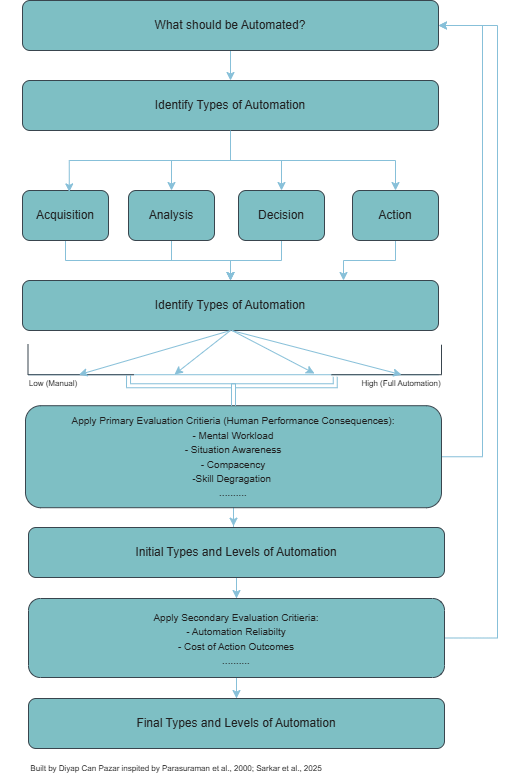
\includegraphics[width=0.60\textwidth]{figures/automation-level.png}

  \caption[Applying types and levels of automation]{Flow chart showing application of the Parasuraman et al.\ model of types and levels of automation. For each automation type (acquisition, analysis, decision, action), a level between low (manual) and high (full automation) is selected and progressively adjusted using primary human-performance consequences and secondary evaluative criteria \parencite{parasuraman2000model}.}

  \label{fig:autonomy-spectrum}

\end{figure}

The primary implication for coding tools is not simply that ``more autonomy is better,'' but that autonomy choices trade off human performance consequences. Parasuraman et al.\ emphasize evaluative criteria such as mental workload, situation awareness, complacency, and skill degradation, alongside reliability and the cost of erroneous actions \parencite{parasuraman2000model}. In an IDE setting, this translates into a concrete tension: higher autonomy can reduce interaction cost (fewer step-by-step exchanges) while increasing the \emph{supervision and verification burden} (larger diffs, fewer intermediate states, higher recovery cost when something drifts).

Despite strong capability, \glspl{llm} display systematic \emph{model-side failure modes}. These include producing code that compiles but violates intended semantics, hallucinating non-existent functions or APIs, and failing to preserve consistency across longer contexts or multi-file edits \parencite{ji2023hallucination, zhang2023sirenssong}. Security risks are particularly salient: AI assistance can raise vulnerability incidence even while developers indicate greater confidence \parencite{perry2023insecure}. Industry-focused evaluations similarly report elevated duplication, inconsistent style, and insufficient error handling in generated code, exposing a gap between ``passes tests'' and production-quality expectations \parencite{qodo2025codequality}.

Equally important are \emph{human-side failure modes}. Prior work documents over-trust and shallow verification strategies in AI-assisted programming, ranging from cursory scanning to more systematic review depending on task stakes and developer experience \parencite{barke2023trust}. More broadly, automation bias deferring to an automated recommendation even when contradictory evidence exists, is a well-established phenomenon in human factors research and transfers directly to coding workflows when outputs appear fluent and plausible \parencite{leeSee2004trust}. These risks are amplified when interaction schemes fragment attention, because interruptions and resumption costs can degrade deliberate reasoning during review \parencite{parnin2011resumption, abad2018taskInterruption}.

Together, these model-side and human-side dynamics motivate the thesis's focus on \emph{verification and visibility}. In many development contexts, the developer is the primary verification mechanism. If intermediate reasoning is hidden, diffs are large, or review time is squeezed by interaction friction, errors can propagate quietly into the codebase. This makes it essential to examine not only whether assistance accelerates tasks, but how different interaction paradigms reshape oversight capacity, workflow stability, and trust calibration \parencite{mozannar2024reading, leeSee2004trust}.

% ---------------------------------------------------------
\section{Vibe Coding as an Interaction Paradigm}
\label{sec:bg-vibe}

\emph{Vibe Coding}, operationalized in this study through GitHub Copilot's Ask mode, is an interaction paradigm in which the developer and the \gls{ai} engage in a turn-by-turn conversational exchange. The developer submits a natural-language prompt describing a desired change, the AI returns a proposed response (e.g., code snippet, explanation, refactoring suggestion), and the developer decides whether and how to integrate it before formulating the next prompt. Each exchange constitutes one interaction cycle; completing a task typically requires multiple cycles. The developer remains the primary agent throughout: deciding what to ask, when to ask, what to apply, and when to move on \parencite[pp.~85--88]{barke2023groundedcopilot}.

Under this paradigm, the human retains direct control over several important dimensions. The developer chooses the scope and specificity of prompts, selects which parts of a response to use, performs integration manually, and initiates test runs. The system does not autonomously modify files or execute commands; every change passes through deliberate developer action. In autonomy terms, this corresponds to lower levels where the system proposes and the human decides and acts \parencite[p.~287]{parasuraman2000model}.

Empirical studies of conversational \gls{ai} tools highlight recurring interaction trends. Barke, James, and Polikarpova describe \emph{acceleration} (speeding up known work) and \emph{exploration} (traversing unfamiliar territory) as two main modes \parencite[pp.~89--95]{barke2023groundedcopilot}. In both, developers iterate: clarifying requirements, refining prompts, and correcting misunderstandings. The practical strength of Vibe Coding is that it preserves high translucency and fine-grained steering: developers see the solution evolve step by step, evaluate increments in isolation, and redirect quickly when outputs drift, supporting continuous trust calibration \parencite{leeSee2004trust}.

The weakness is that this conversational overhead can accumulate across many cycles. When an initial response is incomplete or misleading, developers may enter repeated prompt-and-repair loops, fragmenting workflow and consuming time. Controlled evaluations report that debugging and understanding AI-generated code can offset expected productivity gains in chat-like usage, particularly when verification becomes the bottleneck \parencite{vaithilingam2022expectation, mozannar2024reading}.

% ---------------------------------------------------------
\section{Agentic Coding as an Interaction Paradigm}
\label{sec:bg-agentic}

\emph{Agentic Coding}, operationalized in this study through GitHub Copilot’s Agent mode, is an interaction paradigm in which the developer delegates a goal to an \gls{ai} agent that plans and executes a multi-step sequence to achieve that goal. A common workflow follows a \emph{goal → plan → act → propose → approve} structure: the developer specifies a high-level objective, the agent decomposes it, executes actions (e.g., editing multiple files, running terminal commands, iterating on failing tests), and then surfaces a consolidated result for developer review \parencite{vscodeCopilotAgentMode, sarkar2025codewithme}.

Agent mode goes beyond conversational assistance by combining multi-file context with tool-mediated actions. It is able to navigate and modify several files, invoke shell commands (e.g., running \texttt{pytest}), create new files, and iterate in response to execution feedback before asking the developer for approval \parencite{vscodeCopilotCodingAgent}. Sapkota, Roumeliotis, and Karkee conceptualize agentic coding systems as combining goal interpretation, task decomposition, tool utilization, iterative execution, long-context handling, and self-correction \parencite{sapkota2025vibecoding}. In the configuration described in this thesis, these capabilities are bounded by explicit \emph{approval checkpoints} for potentially impactful operations (e.g., command execution, applying edits). The checkpoint design is central: it preserves human monitoring while still enabling the agent to compress multiple execution steps into fewer interaction cycles \parencite[p.~21]{sarkar2025codewithme}.

\begin{figure}[H]
  \centering
  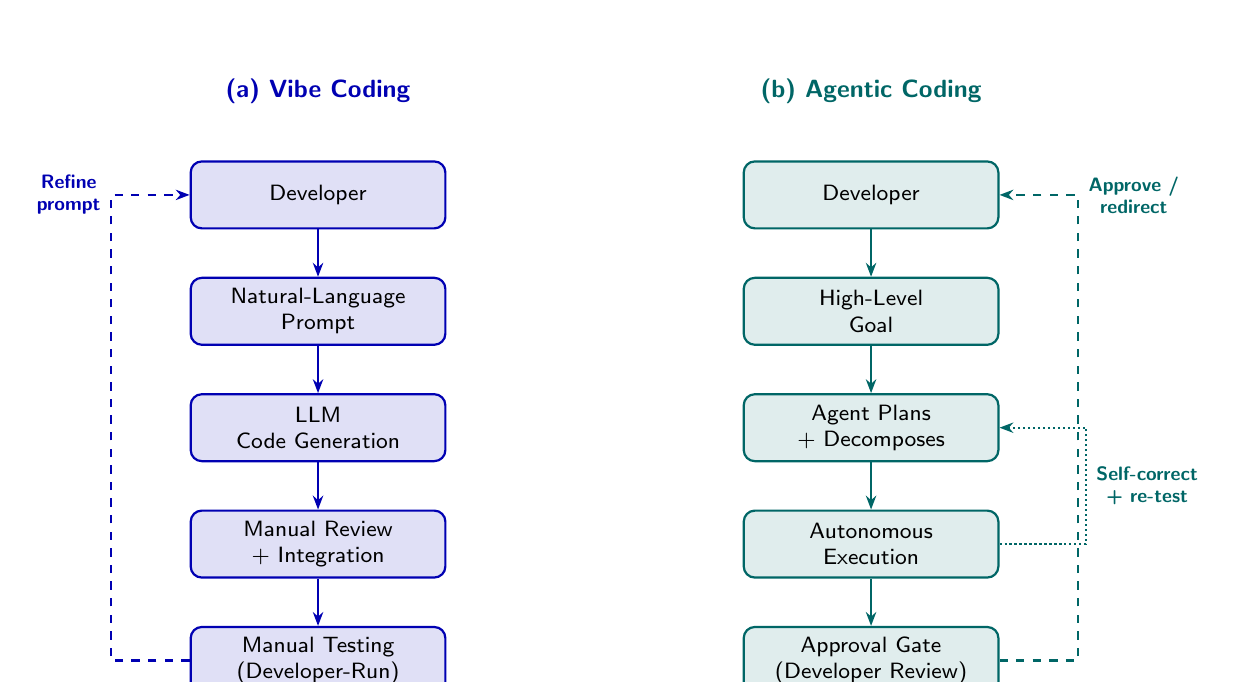
\begin{tikzpicture}[
      font=\footnotesize\sffamily,
      node distance=6mm and 10mm,
      box/.style={rectangle, rounded corners=4pt, draw=#1, fill=#1!12,
      text width=3.0cm, minimum height=8.5mm, align=center, line width=0.8pt},
      arrow/.style={-{Stealth[length=5pt]}, thick, draw=#1},
      title/.style={font=\small\sffamily\bfseries, text=#1},
      lbl/.style={font=\scriptsize\sffamily\bfseries, text=#1}
    ]

    % =======================
    % (a) Vibe Coding (left)
    % =======================
    \node[title=blue!70!black] (titleA) {(a) Vibe Coding};

    \node[box=blue!70!black, below=of titleA] (devA) {Developer};
    \node[box=blue!70!black, below=of devA] (nlA) {Natural-Language\\Prompt};
    \node[box=blue!70!black, below=of nlA] (llmA) {LLM\\Code Generation};
    \node[box=blue!70!black, below=of llmA] (revA) {Manual Review\\+ Integration};
    \node[box=blue!70!black, below=of revA] (testA) {Manual Testing\\(Developer-Run)};

    \draw[arrow=blue!70!black] (devA) -- (nlA);
    \draw[arrow=blue!70!black] (nlA) -- (llmA);
    \draw[arrow=blue!70!black] (llmA) -- (revA);
    \draw[arrow=blue!70!black] (revA) -- (testA);

    % feedback loop (kept outside to avoid collisions)
    \draw[arrow=blue!70!black, dashed]
    (testA.west) -- ++(-1.0,0) |- node[left, lbl=blue!70!black, align=center]{Refine\\prompt} (devA.west);

    % ==========================
    % (b) Agentic Coding (right)
    % ==========================
    % anchor right block relative to left block so width changes don't break it
    \node[title=teal!80!black, right=4.2cm of titleA] (titleB) {(b) Agentic Coding};

    \node[box=teal!80!black, below=of titleB] (devB) {Developer};
    \node[box=teal!80!black, below=of devB] (goalB) {High-Level\\Goal};
    \node[box=teal!80!black, below=of goalB] (planB) {Agent Plans\\+ Decomposes};
    \node[box=teal!80!black, below=of planB] (execB) {Autonomous\\Execution};
    \node[box=teal!80!black, below=of execB] (gateB) {Approval Gate\\(Developer Review)};

    \draw[arrow=teal!80!black] (devB) -- (goalB);
    \draw[arrow=teal!80!black] (goalB) -- (planB);
    \draw[arrow=teal!80!black] (planB) -- (execB);
    \draw[arrow=teal!80!black] (execB) -- (gateB);

    % approval loop (kept outside to avoid collisions)
    \draw[arrow=teal!80!black, dashed]
    (gateB.east) -- ++(1.0,0) |- node[right, lbl=teal!80!black, align=center]{Approve /\\redirect} (devB.east);

    % self-correction loop (clean and readable)
    \draw[arrow=teal!80!black, densely dotted]
    (execB.east) -- ++(1.1,0)
    |- node[right, lbl=teal!80!black, align=center, pos=0.25]{Self-correct\\+ re-test}
    (planB.east);

  \end{tikzpicture}

  \caption[Bird’s-Eye Comparison of Vibe Coding and Agentic Coding]{Bird’s-eye comparison of the two paradigms, adapted from \textcite{sapkota2025vibecoding}. (a)~Vibe Coding: the developer drives each cycle through natural-language prompts, manual integration, and developer-run testing. (b)~Agentic Coding: the developer delegates a high-level goal; the agent plans, executes, and self-corrects autonomously, surfacing results at an approval gate.}
  \label{fig:birdeye-comparison}
\end{figure}

Relative to Vibe Coding, Agentic Coding shifts responsibility from step-by-step steering toward supervisory oversight. In automation terms, the developer monitors outcomes and intervenes at gates rather than directing every action \parencite[pp.~289--291]{parasuraman2000model, vscodeCopilotAgentMode}. This makes \emph{situation awareness} salient: the developer must retain enough understanding of what the agent changed, why it changed it, and what is still uncertain to perform meaningful verification and early intervention \parencite{endsley1995situation}.


Potential strengths follow from \emph{batching}: compressing multi-step work into fewer interaction cycles. Instead of the developer orchestrating each edit and check, the agent can traverse the understand $\rightarrow$ edit $\rightarrow$ run $\rightarrow$ test $\rightarrow$ debug $\rightarrow$ repeat loop and surface a consolidated result. For tasks with clear success criteria (e.g., automated tests), this can reduce interaction cost and shorten completion time, as the agent can iterate internally until it satisfies the oracle \parencite{sarkar2025codewithme}.

Possible weaknesses relate to \emph{visibility loss} and \emph{goal drift}. Because the agent executes multiple steps autonomously, the developer sees fewer intermediate states and might struggle to reconstruct why particular changes were made, especially when edits span several files. When the agent pursues an unproductive direction, errors can compound before the developer notices, increasing recovery cost \parencite{perry2023insecure}. Approval gates lessen these risks but do not remove them: approving a large change set without careful review carries similar risk to approving a complex pull request with insufficient inspection. These dynamics correspond with broader concerns about automation complacency and trust miscalibration in human-machine systems \parencite{leeSee2004trust}.

% ------------------------------------------------------

\section{Collaboration vs Delegation Trade-Off}
\label{sec:bg-tradeoff}

The paradigms above occupy opposing positions on a collaboration--delegation trade-off in human--\gls{ai} interaction. Vibe Coding embodies a \emph{collaboration model}: the developer and the AI work step by step, with continuous visibility and frequent steering, and the developer integrates outputs manually. Agentic Coding embodies a \emph{delegation model}: the developer specifies a goal and entrusts execution to the AI, shifting from implementation toward supervisory oversight. Each position carries characteristic costs and benefits. Collaboration preserves transparency and fine-grained control but imposes conversational overhead. Delegation reduces interaction cost and compresses multi-step work but increases supervision burden and concentrates risk into fewer, higher-impact approvals \parencite{sarkar2025codewithme, parasuraman2000model}.

This trade-off frames the interpretation of the study outcomes. For \gls{rq1}, delegation is expected to reduce interaction cost and completion time by batching work, but may introduce different interruptions if oversight demands become a bottleneck (e.g., reviewing larger diffs or resolving drift). For \gls{rq2}, delegation is expected to redistribute perceived control from incremental steering to approval and intervention. Trust should remain dynamic in both models and anchored to verification signals (e.g., test outcomes), but the stakes of each reliance decision differ: Vibe Coding involves many small accept/reject choices, whereas Agentic Coding concentrates consequences into fewer approvals. These expectations are not formal hypotheses; they provide an analytical frame for the empirical findings in Chapters~\ref{chap:results} and~\ref{chap:discussion}.

\chapter{Related Work and Research Gap}

\label{chap:related-work}

Building on the productivity dimensions introduced in Section~\ref{sec:bg-tradeoff}, prior empirical studies predominantly operationalize metrics such as \emph{task completion time}, \emph{task success rate}, \emph{acceptance rate}, and \emph{perceived productivity} \parencite[pp.~55--58]{ziegler2024measuring, peng2023copilot, vaithilingam2022expectation}. Because these metrics capture distinct aspects of performance, they are not interchangeable: improvements in speed do not necessarily imply gains in correctness, and subjective usefulness may diverge from objectively measured efficiency.

\section{Productivity Evidence for AI Coding Assistants}

\label{sec:rw-productivity}

Across studies, results suggest \gls{ai} assistance can improve certain productivity dimensions, though effect sizes vary with task design and participant population. Peng et al.\ ran a randomized controlled trial ($n=95$) and found Copilot users completed an HTTP server task 55.8\% faster than a control group, with gains strongest among less experienced developers \parencite{peng2023copilot}. Ziegler et al.\ measured Copilot’s impact within GitHub at scale, reporting an inline-suggestion acceptance rate of roughly 30\% and a correlation between acceptance and self-reported productivity \parencite[pp.~57--59]{ziegler2024measuring}. Cui et al.\ reported 20--30\% task-time reductions in field experiments with professional developers for repository-level work, moderated by task complexity and developer experience \parencite{cui2025effectsgenai}. Taken together, these outcomes support the claim that \gls{ai} assistance can produce measurable speed gains, particularly for well-scoped implementation tasks.

However, productivity benefits are not uniform. Vaithilingam, Zhang, and Glassman found that while participants preferred using Copilot, the tool did not significantly improve completion time or success rate in their controlled evaluation \parencite{vaithilingam2022expectation}. Participants reported difficulty debugging and understanding generated code, indicating that verification and comprehension costs can offset generation speed. Mozannar et al.\ complement this through modeling the cognitive cost of \emph{reading, verifying, and repairing} generated output, highlighting that such costs can remain invisible if measurement focuses on suggestion generation rather than the full interaction cycle \parencite{mozannar2024reading}.

Methodological choices help explain these discrepancies \parencite{wohlin2012experimentation}. Task scope varies from short exercises to repository-level tasks necessitating multi-file reasoning; participant populations range from students to professionals; and measurement choices differ on whether they include downstream time spent validating and integrating outputs. Most importantly for this thesis, many studies treat \gls{ai} assistance as a single intervention (AI vs.\ no-AI), rather than examining how different \emph{interaction paradigms} (collaboration vs.\ delegation) within AI-assisted work reshape outcomes under otherwise controlled conditions.

A newer body of evidence starts to quantify the impact of \emph{agentic} assistants in the wild, which is relevant because the field is actively shifting toward more autonomous tool use. He et al.\ estimate the causal impact of adopting Cursor \gls{ide}\footnote{\url{https://github.com/cursor/cursor}; Cursor is an AI code editor and coding agent.} using a difference-in-differences design and report large but transient velocity gains alongside persistent increases in static analysis warnings and code complexity \parencite{he2025cursorDID}. These results yield valuable macro-level signals (velocity--quality trade-offs) but do not isolate how specific interaction structures (e.g., step-by-step chat versus delegated agent runs) drive those outcomes, nor do they capture within-task flow costs or subjective experience.

% ---------------------------------------------------------

\section{Human--AI Interaction in Programming Workflows}

\label{sec:rw-interaction}

Beyond aggregate productivity metrics, a parallel stream of research examines the \emph{interaction dynamics} that unfold when developers work with \gls{ai} coding tools: how developers prompt, steer, verify, and recover when outputs are wrong, and how these behaviors reshape workflow \parencite{barke2023groundedcopilot, mozannar2024reading}.

Barke, James, and Polikarpova conducted a grounded-theory study of programmers using GitHub Copilot ($n=20$) and identified two dominant interaction fields: \emph{acceleration} (speeding up familiar tasks) and \emph{exploration} (traversing unfamiliar territory) \parencite{barke2023groundedcopilot}. In acceleration mode, developers usually adopt rapid accept-or-reject behavior with relatively shallow scrutiny; in exploration mode, they iterate more critically, inspect suggestions more carefully, and use the assistant to probe unfamiliar solution paths. This distinction matters because it implies the same developer may interact with the same assistant in qualitatively different ways depending on confidence, task familiarity, and perceived stakes.

Verification behavior, how developers check whether AI-generated code is correct, has become a central dimension of interaction quality. Barke, Sarkar, and McKay show that developers use strategies ranging from cursory scanning to systematic line-by-line review, determined by task stakes, code complexity, and experience \parencite{barke2023trust}. Mozannar et al.\ further argue that verification and repair introduce substantial hidden overhead that is often missing from simplified productivity narratives \parencite{mozannar2024reading}. Taken together, these studies contest the assumption that AI assistance is straightforwardly additive: time saved in generation can be partially consumed by time spent understanding, validating, and integrating outputs.

Interruptions and context switching also represent a related concern. Development work is cognitively demanding, and interruptions impose resumption costs that may degrade performance and increase error likelihood \parencite{parnin2011resumption}. AI assistants introduce a tool-mediated interruption pattern: developers pause their reasoning to evaluate an AI suggestion, decide whether to accept or modify it, and then re-enter the original problem context. When suggestions are incorrect or demand heavy modification, the evaluative pause expands into a repair cycle that fragments attention. Abad et al.\ show that interruption disruptiveness depends on both duration and cognitive demand, with interruptions requiring active problem-solving being more costly than passive ones \parencite{abad2018taskInterruption}.

While this interaction literature richly characterizes completion and chat-based assistance, evidence is more limited for how interaction features change when assistance becomes more autonomous (agentic). Ross et al.\ document conversational interaction schemes such as clarification, negotiation, and iterative refinement \parencite{ross2023programmer}, but do not examine tool-using agents that execute multi-step actions. Only quite recent conceptual work contrasts conversational ``vibe'' workflows with ''agentic''  workflows across tool integration and execution environments \parencite{sapkota2025vibecoding}, but the treatment is largely conceptual rather than empirical.

A closely related framing comes from ``code-with-me'' versus ``code-for-me'' interaction: Sarkar et al.\ analyze how increasing automation levels shift developer work from direct implementation toward oversight, underlining that productivity gains can be coupled with supervision costs \parencite{sarkar2025codewithme}. This framing coincides with this thesis’s paradigm distinction (collaboration vs.\ delegation), but existing evidence still leaves open how these paradigms differ \emph{within} a single modern IDE tool configuration under supervised conditions.

Finally, emerging repository-mining studies deliver empirical characterization of agentic coding artifacts in practice. Watanabe et al.\ study pull requests generated with an agentic coding tool Claude Code\footnote{\url{https://code.claude.com/docs/en/overview}} across 157 open-source projects, reporting that agent-assisted PRs are frequently used for refactoring, documentation, and testing and are often merged, but still commonly require human revision to meet project standards \parencite{watanabe2025agenticPR}. Yoshioka et al.\ further compare human and agentic PRs and show that review-related factors can differ in how they relate to PR outcomes \parencite{yoshioka2026meaningfulPR}. These studies strengthen the claim that agentic coding is already a real-world phenomenon, while additionally highlighting that they do not instrument micro-level interaction costs (prompts/runs, interruptions) or capture subjective trust/control inside controlled tasks the focus of this thesis.

% ---------------------------------------------------------

\section{Autonomy, Control, and Trust in Human--AI Systems}

\label{sec:rw-autonomy}

The relationship between automation level, human control, and trust has been studied extensively in domains such as aviation, manufacturing, and driving, producing conceptual frameworks which transfer productively to \gls{ai}-assisted programming. Building on the autonomy concepts introduced in Chapter~\ref{chap:background} (see Figure~\ref{fig:autonomy-spectrum}), Parasuraman, Sheridan, and Wickens’ taxonomy highlights that as automation increases, the operator’s role shifts from active controller to monitor, changing demands on attention, situation awareness, as well as readiness to intervene \parencite[pp.~286--291]{parasuraman2000model}.
\begin{table}[ht]

  \centering

  \small

  \renewcommand{\arraystretch}{1.5}

  \rowcolors{2}{gray!10}{white}

  \begin{tabularx}{\textwidth}{p{3.5cm} X}

    \toprule

    \rowcolor{accentblue}

    \textcolor{black}{\textbf{Level \& Role}} & \textcolor{black}{\textbf{Description}} \\

    \midrule

    1. None & The computer offers no assistance; the human must take all decisions and actions. \\

    2. Alternatives & The computer offers a complete set of decision/action alternatives. \\

    3. Narrows & The computer narrows the selection down to a few alternatives. \\

    4. Suggests & The computer suggests one alternative. \\

    5. Executes with Approval & The computer executes that suggestion if the human approves. \\

    6. Veto Period & The computer allows the human a restricted time to veto before automatic execution. \\

    7. Automatic (Inform) & The computer executes automatically, then necessarily informs the human. \\

    8. Inform on Request & The computer informs the human only if asked. \\

    9. Inform if Decided & The computer informs the human only if it decides to. \\

    10. Autonomous & The computer decides everything and acts autonomously, ignoring the human. \\

    \bottomrule

  \end{tabularx}

  \caption{Levels of Automation (adapted from Parasuraman, Sheridan, and Wickens, 2000).}

  \label{tab:levels-of-automation}

\end{table}

Trust calibration, how users adjust reliance on an automated system according to observed performance, is central to effective human automation interaction. Lee and See define trust as the attitude that an agent will help achieve goals under conditions of uncertainty and vulnerability, and propose that trust is determined by \emph{performance}, \emph{process} (transparency), and \emph{purpose} \parencite[pp.~54--62]{leeSee2004trust}. Miscalibration yields two failure modes: over-trust (relying beyond capability) and under-trust (rejecting reliable assistance). Both are relevant to AI-assisted coding: over-trust can lead to accepting incorrect code without sufficient verification, while under-trust can lead to ignoring useful suggestions or micro-managing an effective agent.

System properties that affect trust calibration: transparency, controllability, and predictability, map directly onto the paradigms examined in this thesis. Vibe Coding tends to preserve higher transparency (incremental outputs) and direct controllability (steering each step), which may support calibration. Agentic Coding reduces visibility into intermediate states and shifts controllability to a higher level of abstraction (supervision and intervention), possibly making calibration harder, especially when change sets are large or span multiple files. Sarkar et al.\ formalize this tension by framing AI coding tools along an automation spectrum in which increasing autonomy shifts developer effort from implementation to oversight, and the benefits of higher automation depend on sufficient supervisory skill \parencite{sarkar2025codewithme}. More generally, work on automation bias and complacency argues that increased automation can reduce watchfulness and situation awareness unless monitoring support scales accordingly \parencite{parasuramanManzey2010, endsley1995situation}.

A remaining gap concerns evidence specific to \emph{coding agents} as distinct from chat-based assistants. Many trust and autonomy frameworks come from non-programming domains, and within software engineering, much empirical work focuses on lower-autonomy tools (completion, chat). Tool-using agents that plan, execute, and self-correct across multiple files and commands create distinct oversight dynamics: fewer intermediate checkpoints, higher recovery costs when drift occurs, and approval-gate interaction schemes that concentrate risk into fewer decisions. While field evidence increasingly documents agentic outcomes (e.g., PR acceptance/edits \parencite{watanabe2025agenticPR} and ecosystem-level velocity/quality trade-offs \parencite{he2025cursorDID}), controlled comparisons that link these outcomes to measurable interaction costs and subjective trust/control remain scarce.

\section{Risks and Trade-Offs: Quality, Security, and Over-Reliance}

\label{sec:rw-risks}

Productivity-oriented work is complemented by research documenting risks and unintended consequences of \gls{ai}-assisted coding. Code quality concerns comprise duplication, insufficient error handling, inconsistent naming conventions, and poor adherence to design patterns. The Qodo 2025 State of AI Code Quality report argues that AI-generated code can underperform human-written code on maintainability-related metrics even when it achieves functional correctness \parencite{qodo2025codequality}. These quality gaps are concerning because they may be invisible in short-term evaluations: code that passes tests today may create technical debt or maintenance burden later.

Security risks have received particular empirical attention. Perry et al.\ found that participants with access to an AI assistant produced more security vulnerabilities than a control group while simultaneously expressing higher confidence in their code’s security \parencite{perry2023insecure}. This combination illustrates a dangerous form of trust miscalibration: fluent outputs can create a false sense of correctness, reducing critical scrutiny. The risk is plausibly amplified under agentic workflows where assistants generate larger change sets that are harder to review exhaustively. Complementing controlled studies, ecosystem evidence suggests that agentic adoption can correlate with persistent increases in static analysis warnings and code complexity \parencite{he2025cursorDID}, strengthening the need to treat quality assurance and verification as first-class activities rather than afterthoughts.

Over-reliance ties quality and security concerns together. When developers delegate verification implicitly rather than performing it deliberately, errors and vulnerabilities can propagate. This pattern is directly relevant to \gls{rq2}, which examines how trust and control perceptions differ across paradigms, and to \gls{rq1}, if efficiency gains are partially offset by repair and inspection costs \parencite{mozannar2024reading, vaithilingam2022expectation}. In this thesis, these risks motivate an interaction-focused evaluation that quantifies not only outcomes (time/success) but also the costs of oversight and flow disruption throughout the development process.

Table~\ref{tab:literature-summary} consolidates key empirical and closely related studies reviewed in this chapter. The rightmost column identifies the specific gap each study leaves that the present thesis addresses.

\begin{table}[H]

  \centering

  \caption[Summary of Key Empirical Studies]{Summary of key studies reviewed in this chapter. The rightmost column identifies the gap each study leaves that the present thesis addresses.}

  \label{tab:literature-summary}

  \footnotesize

  \setlength{\tabcolsep}{3pt}

  \renewcommand{\arraystretch}{1.0}

  \rowcolors{2}{gray!10}{white}

  \begin{tabularx}{\textwidth}{>{\raggedright\arraybackslash}p{2.8cm} >{\raggedright\arraybackslash}p{2cm} X >{\raggedright\arraybackslash}p{4cm}}

    \toprule

    \rowcolor{accentblue}

    \textcolor{black}{\textbf{Study}} & \textcolor{black}{\textbf{Method}} & \textcolor{black}{\textbf{Main finding}} & \textcolor{black}{\textbf{Gap addressed here}} \\

    \midrule

    \textbf{Peng et al.} \parencite{peng2023copilot} &

    RCT ($n=95$) &

    Copilot users completed task \textbf{55.8\% faster}; gains strongest for novices. &

    Compares \emph{AI vs.\ no-AI}; not \emph{interaction paradigms}. \\

    \textbf{Ziegler et al.} \parencite{ziegler2024measuring} &

    Field (GitHub) &

    Acceptance rate ($\sim$30\%) correlated with perceived productivity. &

    Focuses on \emph{completion}; excludes chat/agent workflows. \\

    \textbf{Cui et al.} \parencite{cui2025effectsgenai} &

    Field exp.\ ($\times 3$) &

    GenAI reduced time by \textbf{20--30\%}; moderated by complexity/experience. &

    No \emph{within-tool mode} comparison. \\

    \textbf{Vaithilingam et al.} \parencite{vaithilingam2022expectation} &

    Lab &

    Copilot preferred but no time improvement; verification overhead high. &

    No manipulation of autonomy / paradigms within one tool. \\

    \textbf{Barke et al.} \parencite{barke2023groundedcopilot} &

    Qualitative &

    Two styles: \emph{acceleration} and \emph{exploration}. &

    No controlled efficiency/flow comparison across paradigms. \\

    \textbf{Mozannar et al.} \parencite{mozannar2024reading} &

    Cognitive model &

    Verification/repair introduce substantial \emph{hidden overhead}. &

    Costs not compared across autonomy levels (chat vs.\ agent). \\

    \textbf{Perry et al.} \parencite{perry2023insecure} &

    Lab &

    AI increased vulnerabilities while increasing confidence. &

    Does not compare trust/control across paradigms. \\

    \textbf{Sarkar et al.} \parencite{sarkar2025codewithme} &

    Framework + eval. &

    Higher automation shifts effort from implementation to oversight. &

    Not a focused Ask-vs-Agent comparison with flow/interruptions instrumentation. \\

    \textbf{Watanabe et al.} \parencite{watanabe2025agenticPR} &

    Repo mining &

    Agent-assisted PRs are often merged, but many require human revision to meet project standards. &

    Observational; lacks controlled tasks and subjective trust/control measures. \\

    \textbf{Yoshioka et al.} \parencite{yoshioka2026meaningfulPR} &

    Repo mining &

    Human vs.\ agentic PRs show differing effects of review-related factors on outcomes. &

    Observational; not a within-subject comparison of interaction paradigms. \\

    \textbf{He et al.} \parencite{he2025cursorDID} &

    Causal inference (DiD) &

    Cursor adoption yields transient velocity gains and persistent increases in warnings/complexity. &

    Project-level evidence; does not isolate paradigm-level interaction costs or perceptions. \\

    \bottomrule

  \end{tabularx}

\end{table}

% ---------------------------------------------------------

\section{Research Gap and Contribution of This Thesis}

\label{sec:rw-gap}

The literature reviewed above reveals a specific gap addressed by this thesis. Empirical assessments of \gls{ai} coding assistants overwhelmingly compare \gls{ai}-assisted versus unassisted conditions, treating AI support as a binary intervention. Within the \gls{ai}-assisted condition, the \emph{interaction paradigm} of how the developer and \gls{ai} collaborate is typically treated as fixed rather than as an independent variable. Few studies manipulate autonomy \emph{within a single tool} while holding other factors constant (same \gls{ide}, same model configuration, same tasks, same participants). Although recent work begins to characterize agentic coding outcomes in the wild (agentic PRs \parencite{watanabe2025agenticPR, yoshioka2026meaningfulPR} and project-level adoption effects \parencite{he2025cursorDID}), these studies do not provide controlled, within-participant comparisons that connect interaction structure to measurable flow costs and to subjective experience (trust, control, workflow fit).

Existing work also underexplores experiential dimensions. Productivity metrics, time, success, and acceptance rate capture outcomes, but omit how developers experience the interaction: how they manage verification decisions, how they perceive control, and whether the interaction rhythm matches their working style. These experiential dimensions influence adoption and determine whether oversight is thorough or superficial \parencite{barke2023trust, leeSee2004trust}.

This thesis addresses the gap through three contributions. First, it provides a controlled within-subject empirical comparison of two coding paradigms: Vibe Coding and Agentic Coding, within a single \gls{ide} (GitHub Copilot in Visual Studio Code), using a fixed \gls{llm} configuration and counterbalanced task assignments to isolate the paradigm variable. Second, it integrates quantitative efficiency and flow measures (time, success, interaction cost, interruptions) with qualitative perception data (trust, control, workflow fit) to capture both what happens and how it is experienced. Third, it translates results into actionable best practices for programmers and companies adopting \gls{ai} coding tools, grounding recommendations in observed empirical trade-offs rather than general claims.

The next chapter details the experimental design, participant recruitment, task materials, and instruments that operationalise these contributions into a concrete research protocol.

\chapter{Methodology} % Target: 3300w
\label{chap:methodology}

\section{Research Design} % Target: 450w

\label{sec:research-design}

% Q1: What is the study design in one sentence (within-subject; two modes; two tasks)? (60w)

% Q2: What are the independent variables (mode; task group) and what is held constant? (90w)

% Q3: What are dependent measures for RQ1 vs RQ2 (high level)? (90w)

% Q4: How does the within-subject flow work for one participant (sequence)? (90w)

% Q5: What is counterbalancing and what bias does it control? (70w)

% Q6: Why include two task groups at design level (task-type sensitivity)? (50w)

In this chapter we operationalize the paradigm distinction developed in Chapters~\ref{chap:background} and~\ref{chap:related-work}. Building on the conceptual differentiation between collaborative (Vibe) and delegated (Agent) development approaches, it specifies how these modes were translated into an empirical study design. Emphasis changes from theoretical framing to empirical implementation, detailing task structure, controlled variables, measurement instruments, and data collection procedures used to isolate the factors influencing the interaction style on developer efficiency and perception.

The study design draws on established empirical approaches for evaluating AI-assisted programming tools. Prior work contrasting collaborative and more autonomous assistance paradigms informed the framing of interaction styles \parencite[p.~5]{sarkar2025codewithme}, while research on trust and perception in AI-generated code motivated the inclusion of perceptual measures alongside performance outcomes \parencite[pp.~3--5]{barke2023trust}. Following experimental design guidance in software engineering, a within-subject design was selected to reduce variance stemming from individual differences such as programming proficiency, problem-solving style, and prior AI exposure \parencite{wohlin2012experimentation}.

The interaction paradigm (Vibe vs.\ Agentic) constitutes the primary independent variable. Task type functions as a secondary design factor through two task groups (TG1/TG2), later described in Section~\ref{sec:tasks-and-materials}. Across paradigms, the workflow frame remains constant: participants worked in the same IDE, used the same repository structure, received identical task instructions within their assigned group, and were evaluated using the same test-based success oracle. This configuration isolates interaction style as the central source of experimental variation.

Dependent measures align directly with the research questions. For RQ1, efficiency and flow are captured through task achievement/completion time, task success, interaction cost proxies (e.g., prompts or agent runs), and coded interruption episodes (Section~\ref{sec:measures}). For RQ2, perceptions are measured immediately after each task using Likert-scale items (trust, perceived control, workflow fit, perceived difficulty) and further explored in short semi-structured interviews (Section~\ref{sec:procedure}).

To mitigate order effects, paradigm order was counterbalanced: half of the participants completed their first task in Vibe mode and their second in Agentic mode, while the remainder followed the reverse sequence. This reduces practice and carryover effects, strengthening internal validity \parencite{wohlin2012experimentation}.

\section{Participants} % Target: 500w
\label{sec:participants}
% Q1: Who participated (n, experience strata) and why balanced. (90w)
% Q2: Inclusion criteria (Python/experience) and rationale. (90w)
% Q3: Recruitment method and potential sampling bias. (70w)
% Q4: Copilot experience distribution and why recorded. (90w)
% Q5: Allocation across task group and mode order (balanced). (80w)
% Q6: Consent/recording/pseudonymization steps. (80w)

Excluding participants involved in the pilot study, 12 participants ($n=12$) took part in the research, spanning heterogeneous levels of professional software development experience. To avoid the sample being dominated by one seniority level, participants were stratified into three equally sized experience groups: junior ($n=4$), mid-level ($n=4$), and senior ($n=4$). This enables interpreting whether paradigm-related effects appear consistently across experience levels, including potential differences in verification habits and comfort with delegation.

Recruitment followed basic inclusion criteria: prior programming experience, familiarity with Python, and prior exposure to AI-assisted coding tools. Participants were not filtered by AI-tool expertise level, since variation in familiarity was treated as analytically meaningful rather than noise to eliminate. Baseline familiarity with GitHub Copilot was recorded on a five-point self-report scale. Across the sample, Copilot experience showed a mean of $M=3.0$ ($SD=1.35$), a median of $3$, and ranged from $1$ to $5$ (distribution: 1: $n=1$, 2: $n=4$, 3: $n=4$, 4: $n=0$, 5: $n=3$). Sessions were recorded (screen and audio) with consent and stored under pseudonymous identifiers (P1--P12) (Section~\ref{sec:data-collection}).

Participant allocation balanced two factors across experience levels: (1) paradigm order and (2) task group membership (TG1/TG2). Table~\ref{tab:counterbalancing} summarizes placement across task group, paradigm order, and experience level. Task groups and materials are detailed in Section~\ref{sec:tasks-and-materials}; the assignment here is reported only to document counterbalancing.

\begin{table}[H]
  \centering
  \caption[Participant Allocation]{Participant placement across task group, paradigm order, and experience level.}
  \label{tab:counterbalancing}
  \renewcommand{\arraystretch}{1.15}
  \rowcolors{2}{gray!10}{white}
  \begin{tabular}{c l l c}
    \toprule
    \rowcolor{accentblue}
    \textbf{Participant} & \textbf{Task Group} & \textbf{Paradigm Order} & \textbf{Experience Level} \\
    \midrule
    P1  & TG1 -- Data analysis & Vibe $\rightarrow$ Agentic & Junior \\
    P2  & TG1 -- Data analysis & Agentic $\rightarrow$ Vibe & Junior \\
    P3  & TG1 -- Data analysis & Vibe $\rightarrow$ Agentic & Mid-level \\
    P4  & TG1 -- Data analysis & Agentic $\rightarrow$ Vibe & Mid-level \\
    P5  & TG1 -- Data analysis & Vibe $\rightarrow$ Agentic & Senior \\
    P6  & TG1 -- Data analysis & Agentic $\rightarrow$ Vibe & Senior \\
    P7  & TG2 -- Bug fixing    & Vibe $\rightarrow$ Agentic & Junior \\
    P8  & TG2 -- Bug fixing    & Agentic $\rightarrow$ Vibe & Junior \\
    P9  & TG2 -- Bug fixing    & Vibe $\rightarrow$ Agentic & Mid-level \\
    P10 & TG2 -- Bug fixing    & Agentic $\rightarrow$ Vibe & Mid-level \\
    P11 & TG2 -- Bug fixing    & Vibe $\rightarrow$ Agentic & Senior \\
    P12 & TG2 -- Bug fixing    & Agentic $\rightarrow$ Vibe & Senior \\
    \bottomrule
  \end{tabular}
\end{table}

This allocation reduces the likelihood that observed differences between paradigms arise from systematic ordering patterns or experience-level imbalance rather than the interaction paradigm itself.
\section{Tools and Experimental Setup}
\label{sec:tools-setup}

The experimental arrangement follows a simple principle: keep the surrounding workflow constant, and vary only the interaction paradigm. All participants worked in Microsoft Visual Studio Code (version~1.108) on a shared GitHub repository\footnote{\url{https://github.com/hm-study-copilot-B/copilot-vibe-agentic-coding-study/}}, ensuring identical task files, prompts, and project structure across sessions. Code execution and evaluation were performed locally via an integrated terminal, with task achievement determined through automated \texttt{pytest} tests \parencite{pytestDocs}.

GitHub Copilot Pro was selected because it supports modes corresponding to both paradigms in the same \gls{ide}, reducing confounds from switching tools or adapting to different UI conventions. In the study configuration, Ask mode was used for conversational prompting and code suggestions, while Agent mode was used for goal-level delegation with multi-step execution support. Capabilities were treated at the level of what the tool was by default allowed to do (e.g., participants always retained approval for consequential actions), and are summarized in Table~\ref{tab:copilot-modes} \parencite{githubCopilotFeatures,vscodeCopilotAgentMode,vscodeCopilotCodingAgent,githubAgentMode101}.

To avoid confounding interaction paradigm with model capability, Copilot’s selected \gls{llm} was held constant across sessions. The study used Claude Sonnet~4.5\footnote{\url{https://www.anthropic.com/news/claude-sonnet-4-5}} throughout, and the model configuration was not changed mid-study to preserve internal validity \parencite{githubCopilotDocs,anthropicSonnet45}. Benchmark work such as SWE-bench motivates why repository-scale tasks evaluated by test oracles are a relevant reference point for model/tool selection, even though the present study concentrates on interaction structure rather than model ranking \parencite{sweBenchmark, sweBench}.

Python was used as the task language because it supports both task categories employed here (data analysis and bug fixing) while remaining accessible across experience levels. Automated tests provided a consistent correctness oracle across paradigms \parencite{pytestDocs}.

\begin{table}[H]
  \centering
  \caption[Coding-Paradigm Capabilities]{Capabilities of the two coding paradigms as operationalized through GitHub Copilot in the study environment. Vibe Coding maps to Copilot's Ask mode; Agentic Coding maps to Copilot's Agent mode. \cmark\;denotes the capability is supported directly, $\cmark^{\dagger}$ denotes support that typically requires explicit developer approval (e.g., before applying edits or executing terminal commands), and \xmark\;denotes that the capability was not available in that interaction paradigm during the study \parencite{githubCopilotFeatures,vscodeCopilotAgentMode,vscodeCopilotCodingAgent}.}
  \label{tab:copilot-modes}
  \renewcommand{\arraystretch}{1.25}
  \rowcolors{2}{gray!10}{white}
  \begin{tabular}{p{2.8cm}cc|cccc}
    \toprule
    \rowcolor{accentblue}
    \textbf{Coding Paradigm} &
    \multicolumn{2}{c}{\textbf{Core Assistance}} &
    \multicolumn{4}{c}{\textbf{Extended Execution Capabilities}} \\
    \cmidrule(lr){2-3}\cmidrule(lr){4-7}
    &
    \textbf{Auto-complete} &
    \textbf{Chat} &
    \textbf{Multi-file} &
    \textbf{Terminal} &
    \textbf{File} &
    \textbf{Act} \\
    &
    &
    &
    \textbf{editing} &
    \textbf{execution} &
    \textbf{creation} &
    \textbf{agentic} \\
    \midrule
    Vibe Coding (Ask mode)
    & \cmark
    & \cmark
    & $\cmark^{\dagger}$
    & \xmark
    & \xmark
    & \xmark \\
    Agentic Coding (Agent mode)
    & \cmark
    & \cmark
    & \cmark
    & $\cmark^{\dagger}$
    & \cmark
    & $\cmark^{\dagger}$ \\
    \bottomrule
  \end{tabular}
\end{table}

\section{Tasks and Materials}
\label{sec:tasks-and-materials}

To compare the two coding paradigms under regulated yet realistic conditions, the study used repository-based programming tasks. In this thesis, a \emph{task} refers to a time-boxed assignment performed within the provided GitHub repository (Section~\ref{sec:tools-setup}): participants modify starter code to satisfy stated requirements and validate progress by running an automated \texttt{pytest} test suite \parencite{pytestDocs}. Each participant completed two tasks (Task~A and Task~B) within a single assigned task group, using one coding paradigm per task. The mapping of paradigms to Task~A versus Task~B follows the counterbalanced procedure described in Section~\ref{sec:procedure}.

Two task categories were selected to represent distinct development activities. Task Group~1 (TG1) consists of GAIA-inspired data analysis tasks \parencite[p.~4]{gaiaBenchmark}. Task Group~2 (TG2) consists of SWE-bench-inspired bug-fixing tasks \parencite[p.~3--8]{sweBenchmark}. Both categories are implemented as Python repository tasks, but vary in cognitive demand: TG1 emphasizes exploration and interpretation, whereas TG2 emphasizes tracing failures and implementing minimal, high-precision fixes. This contrast supports examining whether paradigm effects vary with task characteristics \parencite{sarkar2025codewithme,barke2023trust}.

Comparability across coding paradigms was enforced at the material level. Participants received identical written instructions, consistent starter code structure, and equivalent automated tests across conditions. The task prompt and success oracle (tests) remained unchanged between paradigms; only the interaction paradigm used to obtain AI assistance differed.

\subsection{Repository Structure and Provided Materials}

At the start of each session, participants received the repository address (Section~\ref{sec:tools-setup}). Each task (A or B) was contained in its own folder and included (1) starter code in \texttt{src/}, (2) a test suite in \texttt{tests/}, and (3) task-specific input files where relevant (e.g., a CSV file for data analysis tasks). Figure~\ref{fig:repo-structures} summarizes the repository layout as presented to participants.

\begin{figure}[H]
  \setlength{\fboxsep}{5pt}
  \centering
  \begin{minipage}[t]{0.44\textwidth}
    \fbox{%
      \parbox{\textwidth}{\footnotesize
        \textbf{Task Group 1 (TG1): Data analysis tasks}\par\medskip
        \texttt{task\_group\_1/}\\
        \texttt{├─ task\_1a/}\\
        \texttt{│\ \ ├─ README.md}\\
        \texttt{│\ \ ├─ data/ \ \ \ \ \ (CSV)}\\
        \texttt{│\ \ ├─ src/ \ \ \ \ \ (solution.py)}\\
        \texttt{│\ \ └─ tests/ \ \ (test\_solution.py)}\\
        \texttt{└─ task\_1b/}\\
        \texttt{\hspace*{1.6em}├─ README.md}\\
        \texttt{\hspace*{1.6em}├─ data/ \ \ \ \ \ (CSV)}\\
        \texttt{\hspace*{1.6em}├─ src/ \ \ \ \ \ (solution.py)}\\
        \texttt{\hspace*{1.6em}└─ tests/ \ \ (test\_solution.py)}\\
    }}
  \end{minipage}
  \hspace{1.2em}
  \begin{minipage}[t]{0.44\textwidth}
    \fbox{%
      \parbox{\textwidth}{\footnotesize
        \textbf{Task Group 2 (TG2): Bug-fixing tasks}\par\medskip
        \texttt{task\_group\_2/}\\
        \texttt{├─ task\_2a/}\\
        \texttt{│\ \ ├─ README.md}\\
        \texttt{│\ \ ├─ src/ \ \ \ \ \ (solution.py, demo.py)}\\
        \texttt{│\ \ └─ tests/ \ \ (test\_solution.py)}\\
        \texttt{└─ task\_2b/}\\
        \texttt{\hspace*{1.6em}├─ README.md}\\
        \texttt{\hspace*{1.6em}├─ src/ \ \ \ \ \ (solution.py, demo.py)}\\
        \texttt{\hspace*{1.6em}└─ tests/ \ \ (test\_solution.py)}\\
        \texttt{\hspace*{1.6em}}\\
        \texttt{\hspace*{1.6em}}\\
    }}
  \end{minipage}

  \caption[Repository Structure for TG1 \& TG2]{Repository structure provided to participants. Each participant completed Task~A and Task~B within their assigned task group (TG1 or TG2).}
  \label{fig:repo-structures}
\end{figure}

\subsection{Task Descriptions}
\label{sec:task-desc}

In TG1 (Tasks~1A and 1B), participants worked with a CSV dataset and implemented the required analysis logic in \texttt{src/solution.py}. The tasks were testable through an automated suite, enabling objective correctness checks while still requiring iterative reasoning and interpretation. The exact codes for Task~1A and Task~1B are reproduced in Appendix~\ref{app:tg1a-code} and Appendix~\ref{app:tg1b-code}.

In TG2 (Tasks~2A and 2B), participants were presented with an existing implementation containing bugs and were asked to fix the code so that the supplied \texttt{pytest} suite passes \parencite{pytestDocs}. Running the tests surfaced failing cases and error messages, supporting a debugging workflow centered on localized code comprehension and precise modifications. The exact prompts and code context for Task~2A and Task~2B are reproduced in Appendix~\ref{app:tg2a-code} and Appendix~\ref{app:tg2b-code}.

\subsection{Success Criteria, Difficulty Selection, and Constraints}
\label{sub:success-criteria}
Task achievement was defined as passing all provided \texttt{pytest} tests within the fixed time limit. If the time limit was reached before all tests passed, the task was recorded as incomplete; partial progress (code state and latest test outcome) was retained for analysis.

Task difficulty was calibrated through pilot sessions to reduce ceiling and floor effects. Piloting verified that tasks are solvable within the time box with meaningful effort, not trivial without deliberate reasoning, and not systematically unsolvable under either paradigm. Based on these pilots, task wording and tests were refined to ensure an unambiguous target behavior while preserving non-trivial workload \parencite{wohlin2012experimentation}.

To decrease external variance and contamination, participants were prohibited from consulting the internet and were instructed not to use any \gls{ai} tools other than the configured GitHub Copilot mode assigned for the task. Participants were also instructed not to consult colleagues or friends during the session.

\section{Procedure}
\label{sec:procedure}

Each session followed an identical end-to-end structure to maintain comparability across participants. After a brief onboarding and environment check, participants completed two tasks (Task~A and Task~B) within their assigned task group (Section~\ref{sec:task-desc}). The two tasks were completed under different coding paradigms (Vibe Coding vs.\ Agentic Coding). Immediately after each task, participants completed a brief post-task questionnaire capturing paradigm-specific perceptions (Likert items documented in Appendix~\ref{app:master-thesis}). The session concluded with a short semi-structured interview focusing on contrasts between paradigms and notable moments observed during task execution.

\begin{table}[ht]

  \centering

  \caption{Session Structure and Time Allocation per Participant}

  \label{tab:session-timing}

  \renewcommand{\arraystretch}{1.2}

  \rowcolors{2}{gray!10}{white}

  \begin{tabular}{p{11cm}r}

    \toprule

    \rowcolor{accentblue}

    \textbf{Session Phase} & \textbf{Duration (min.)} \\

    \midrule

    Introduction and Setup & 5--10 \\

    Coding Task 1 & 15 \\

    Post-task Likert Questionnaire (Task 1) & 5 \\

    Coding Task 2 & 15 \\

    Post-task Likert Questionnaire (Task 2) & 5 \\

    Semi-Structured Interview & 10--15 \\

    \midrule

    \textbf{Total} & \textbf{45--60} \\

    \bottomrule

  \end{tabular}

\end{table}

Standardization was enforced using a fixed briefing script and checklist applied at the start of every session. Participants were reminded of the common success criterion (passing the provided \texttt{pytest} tests) and instructed to read the task-specific \texttt{README.md} before beginning each task.

Paradigm switching was implemented as a clean transition between Task~A and Task~B to reduce carryover from earlier context. Each task resided in its own folder with independent starter code and tests. When moving to the second task, participants opened the new task folder and began a fresh Copilot interaction for that paradigm (i.e., without relying on prior chat context).

Each coding task was time-boxed to 15 minutes (Table~\ref{tab:session-timing}). If the time limit was reached before all tests passed, the task was stopped and marked as incomplete. Partial progress was retained (code state, latest test outcomes, and recording), enabling later analysis of where progress stalled and how the paradigm shaped recovery attempts.

Carryover effects were mitigated through three safeguards: (1) paradigm order was counterbalanced across participants, (2) each participant worked within only one task group (TG1 or TG2), and (3) task separation was enforced structurally (distinct folders, prompts, and tests).

\section{Measures and Instruments}
\label{sec:measures}

Measures were selected to map directly to the research questions: performance and workflow disruption for RQ1, and perceived trust/control/workflow fit for RQ2. Definitions of the underlying constructs are provided in Chapters~\ref{chap:background}--\ref{chap:related-work}; this section focuses on operationalization.

\paragraph{Task completion time (RQ1).}
Completion time was defined as the elapsed time between task start (first code edit or Copilot interaction after opening the task folder) and the first point at which all \texttt{pytest} tests passed. If the time limit was reached, time was recorded as the full time box with an incomplete outcome (0/1). Timing was derived from session recordings and corroborated via visible test runs and task transitions.

\paragraph{Task achievement (RQ1).}
Task achievement was operationalized as functional correctness according to the provided \texttt{pytest} suite: a task was successful only if all tests passed within the time limit. This provides a paradigm-invariant success oracle and reduces ambiguity in what counts as ``done'' \parencite{sweBenchmark,pytestDocs}.

\paragraph{Interaction cost (RQ1).}
Interaction cost captures the amount of explicit assistance-seeking required. In Vibe/Ask, this is operationalized as the number of user prompting cycles (prompts and follow-ups). In Agentic/Agent, this is operationalized as the number of agent runs and required approvals. Counts were derived from screen recordings and session notes.

\paragraph{Interruptions and flow breaks (RQ1).}
Interruptions were captured by structured observational coding aligned to recordings. An interruption was coded when visible progress paused for a sustained period due to uncertainty, tool friction, or recovery work (e.g., extended rereading, repeated undoing/backtracking, or prolonged stalling before the next actionable step). This treats interruption episodes and resumption effort as indicators of workflow disruption \parencite{parnin2011resumption,abad2018taskInterruption,meyer2014productivity}.

\paragraph{Post-task perceptions (RQ2).}
After each task, participants completed short Likert-scale items capturing perceived trust in the assistance, perceived control/oversight, perceived workflow fit, and perceived effort/difficulty. Items were intentionally brief to reduce disruption while still capturing immediate paradigm-specific impressions \parencite{likert1932technique,barke2023trust}.

\paragraph{Semi-structured interview (RQ2).}
A short semi-structured interview elicited explanations behind ratings and surfaced contrasts not captured in numeric responses. Recordings and notes provided behavioral grounding (e.g., verification patterns, hesitation, explicit handoffs, manual takeover), supporting triangulation between enacted behavior and self-report \parencite{wohlin2012experimentation}.

\section{Data Collection and Management}
\label{sec:data-collection}

Data collection combined interaction traces, performance artifacts, and self-reports. Screen and audio recordings captured prompts, Copilot outputs, code edits, terminal/test runs, and visible verification activities across the full session. For each task, the final code state and the last observed test outcome were retained as primary performance artifacts. Post-task questionnaires produced paradigm-specific perception data, and the concluding interview provided comparative reflections that contextualize numeric ratings (Section~\ref{sec:procedure}).

In parallel, a structured and reformatted Excel spreadsheet (\texttt{master\_thesis.xls}; see Appendix~\ref{app:master-thesis}) was maintained to register quantitative measures and structured observational notes (e.g., hesitation, reversals, confusion about tool behavior, manual takeover). These notes support later coding of interruptions and provide context to understand success/failure patterns.

All materials were stored under pseudonymous participant identifiers (P1--P12). Recordings, notes, and questionnaire exports were saved in a secure study directory with restricted access. Identifying information was separated from analysis files, and reporting uses only pseudonyms and avoids personally identifying details in quotations.

\section{Ethical Aspects}
\label{sec:ethics}

Participants received an information post describing the study purpose, procedure, and data administration. They were informed that the session would be screen- and audio-recorded and that participation was voluntary with the right to discontinue at any time without consequence. Data were stored under pseudonymous identifiers (P1--P12), and identifying information was kept separate from analysis artifacts (Section~\ref{sec:data-collection}). Access to raw recordings and exports was restricted to the researcher, and no personally identifying information is reported in the thesis.

\chapter{Results}
\label{chap:results}

\section{Data Preparation and Overview}

The empirical findings are based on all documented  sessions (Python programming tasks with GitHub Copilot and follow-up interviews). No sessions required exclusion due to technical failures or protocol violations. Each participant completed two tasks under two coding paradigms (Section~\ref{sec:tasks-and-materials}), yielding 24 task-level observations.

For analysis, observations were organized into a task-level dataset (24 rows) for overall comparisons and a paired participant-level dataset (12 rows, one observation per paradigm per participant) for within-participant tests. All measures and coding rules follow Section~\ref{sec:measures}; the protocol yielded complete data across all variables.

The quantitative findings (RQ1) are reported in Section~\ref{sec:rq1}, covering completion time, task success, interaction cost, and interruptions. The perceptual findings (RQ2) are reported in the qualitative results section, combining post-task Likert ratings with interview data on trust, control, and workflow fit.

\section{Quantitative Results (RQ1: Efficiency and Flow)}
\label{sec:rq1}

Research Question~1 (RQ1) asked: \emph{How do Vibe Coding and Agentic Coding differ in terms of developer efficiency and flow during programming tasks?} Four metrics were examined: completion time, task achievement, interaction cost, and interruption frequency.

A recurring behavioral pattern that contextualizes multiple RQ1 metrics was the \emph{prompt-and-repair cycle} characteristic of Vibe Coding: participants would submit a prompt, receive a response, run tests, find that the response did not completely resolve the issue, and then pause to formulate a refined follow-up prompt. When repeated, these cycles fragmented the workflow and consumed time. Agentic Coding, by contrast, bundled multiple actions (analysis, edits, and test execution) into single agent runs, reducing the number of discrete exchanges.

\begin{table}[H]

  \centering

  \caption[Overview of RQ1 outcomes by paradigm]{Overview of RQ1 outcomes by coding paradigm across all $n=12$ participants (one task per paradigm per participant). Both mean (SD) and median [Q1,~Q3] are reported for completion time because the small sample and right-censored observations (tasks reaching the time limit) make the median a more robust central-tendency estimate, while the mean facilitates comparison to prior studies. Interaction cost and interruptions are \textbf{counts per task}.}

  \label{tab:rq1-overview}

  \renewcommand{\arraystretch}{1.15}

  \rowcolors{2}{gray!10}{white}

  \begin{tabular*}{\textwidth}{@{}>{\raggedright\arraybackslash}p{0.60\textwidth}cc}

    \toprule

    \rowcolor{accentblue}

    \textbf{Outcome} & \textbf{Vibe Coding} & \textbf{Agentic Coding} \\

    \midrule

    Completion time (min; mean, SD) & 11.2 (4.4) & 6.0 (4.5) \\

    Completion time (min; median [Q1, Q3]) & 12.5 [8.0, 15.0] & 4.6 [2.0, 8.2] \\

    Task success (tasks; \%) & 5/12 (42\%) & 9/12 (75\%) \\

    Interaction cost (count; median [Q1, Q3]) & 5.0 [4, 6] & 1.5 [1, 3] \\

    Interruptions (count; median [Q1, Q3]) & 1.0 [0, 1] & 0.0 [0, 0] \\

    \bottomrule

  \end{tabular*}

\end{table}

\subsection{Completion Time}
\label{sec:completion}

The aggregate results showed a substantial time advantage for Agentic Coding. Across all twelve participants, the median completion time under Agentic Coding was 4.6 minutes (interquartile range [2.0, 8.2]), compared to 12.5 minutes under Vibe Coding (interquartile range [8.0, 15.0]). The mean completion time followed a similar pattern: 6.0 minutes (SD = 4.5) versus 11.2 minutes (SD = 4.4). When assessed as paired within-participant comparisons, Agentic Coding reduced completion time by an average of 5.1 minutes (95\% confidence interval [$-9.1$, $-1.2$]) relative to Vibe Coding. A Wilcoxon signed-rank test confirmed that this reduction was statistically significant ($V=10$, $p=0.020$, rank-biserial $r=0.74$, denoting a large effect).

However, the magnitude of this time advantage was not uniform across task types. As visualized in Figure~\ref{fig:completion_time}, the effect was notably marked in TG1 (data analysis tasks), where Vibe Coding participants more frequently approached the time limit. In TG2 (bug fixing tasks), both paradigms performed well, but Agentic Coding still completed tasks faster (Table~\ref{tab:rq1-by-taskgroup}).

\begin{figure}[H]
  \centering
  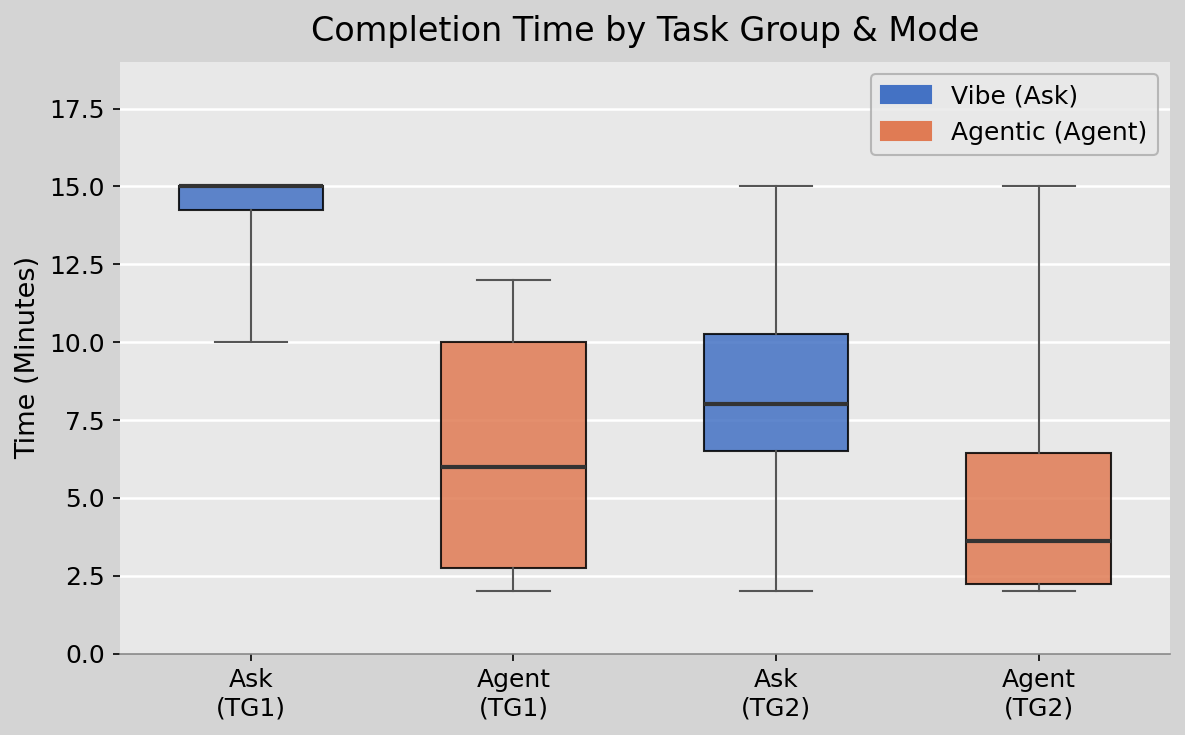
\includegraphics[width=0.8\textwidth]{figures/fig1_time.png}
  \caption[Completion Time by Task Group \& Paradigm]{Distribution of completion times by task group and coding paradigm. Agentic Coding shows consistently lower median times. In TG1, Vibe Coding times cluster near the 15-minute ceiling, reflecting frequent time-limit exhaustion; in TG2, both paradigms performed more similarly, though Agentic Coding retained a time advantage.}
  \label{fig:completion_time}
\end{figure}

\begin{table}[H]

  \centering

  \caption[RQ1 outcomes by task group]{RQ1 outcomes split by task group (TG1: data analysis; TG2: bug fixing). Completion time is in \textbf{minutes}. Each cell has $n=6$ observations.}

  \label{tab:rq1-by-taskgroup}

  \renewcommand{\arraystretch}{1.15}

  \rowcolors{2}{gray!10}{white}

  \begin{tabular*}{\textwidth}{@{\extracolsep{\fill}}llcc}

    \toprule

    \rowcolor{accentblue}

    \textbf{Task Group} & \textbf{Paradigm} & \textbf{Time (min; median [Q1, Q3])} & \textbf{Success (tasks; \%)} \\

    \midrule

    TG1 (Data analysis) & Vibe Coding & 15.0 [14.2, 15.0] & 2/6 (33\%) \\

    TG1 (Data analysis) & Agentic Coding & 6.0 [2.8, 10.0] & 4/6 (67\%) \\

    TG2 (Bug fixing) & Vibe Coding & 8.0 [6.5, 10.2] & 3/6 (50\%) \\

    TG2 (Bug fixing) & Agentic Coding & 3.6 [2.2, 6.5] & 5/6 (83\%) \\

    \bottomrule

  \end{tabular*}

\end{table}

\subsection{Task Success and Failure Cases}

Overall, Agentic Coding yielded a higher task success rate than Vibe Coding (Agentic: 9/12, 75\%; Vibe: 5/12, 42\%). Figure~\ref{fig:success_rates} shows the same pattern when stratified by task group: Agentic Coding achieved higher success in both TG1 (data analysis) and TG2 (bug fixing), with the gap being more pronounced in TG1.

\begin{figure}[H]
  \centering
  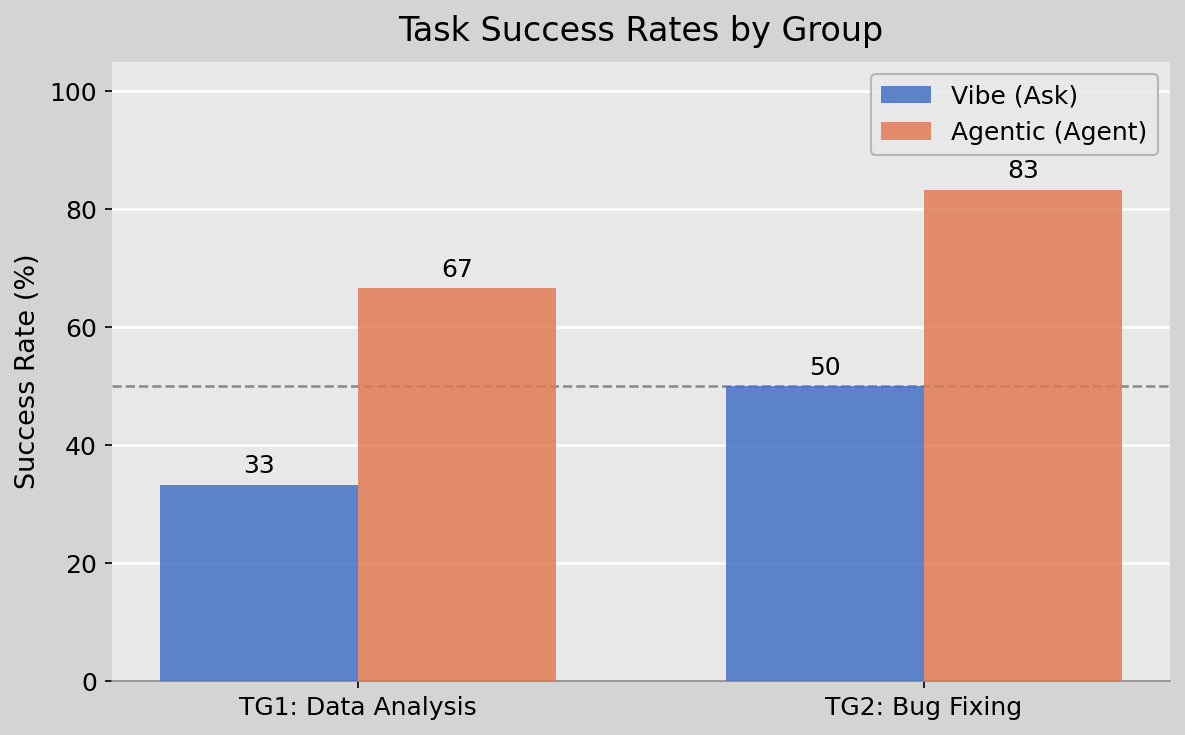
\includegraphics[width=0.7\textwidth]{figures/fig2_success.png}
  \caption[Task Success Rates]{Task success rates by task group. Bars show the percentage of tasks completed successfully within the time limit. Agentic Coding outperforms Vibe Coding in both task groups, with the advantage more pronounced in TG1. Each cell has $n=6$ observations.}
  \label{fig:success_rates}
\end{figure}

When viewed at the level of individual participants, six succeeded only under Agentic Coding, two succeeded only under Vibe Coding, three succeeded in both, and one failed in both. An exact McNemar test on the discordant pairs did not reach significance ($p=0.289$), consistent with the limited sample size.

Failure patterns differed by task group. In TG1, all four Vibe Coding failures coincided with the time ceiling, reflecting sustained prompt-and-repair cycles that prevented convergence on a correct implementation. Agentic Coding failures in TG1 were associated with environment or early-execution faults that consumed setup time. In TG2, Vibe Coding produced three failures, predominantly linked to accumulated implementation errors or environment issues that could not be resolved within the time limit. The single Agentic Coding failure in TG2 was similarly attributable to environment setup overhead rather than conceptual difficulty.

Partial progress was not quantified in the binary success metric, but session recordings captured intermediate states (e.g., reductions in failing tests) that informed the qualitative interpretation of failure cases.

\subsection{Interaction Cost: Prompts and Agent Runs}

Interaction cost captures the granularity of the work process: how many discrete interaction cycles were required to move from the initial task state to a solution (or to the time limit). Under Vibe Coding, each unit was a distinct prompt submitted by the participant; under Agentic Coding, each unit was an agent run (with review/approval decisions). Because one agent run can bundle multiple steps that would require several prompts in Vibe Coding, the comparison is interpreted as the number of discrete human--AI interaction cycles rather than a one-to-one mapping between prompts and runs.

As illustrated in Figure~\ref{fig:interaction_cost}, Agentic Coding required markedly fewer interaction units. The median was 1.5 runs (interquartile range [1, 3]) versus 5.0 prompts under Vibe Coding (Table~\ref{tab:rq1-overview}). A paired Wilcoxon signed-rank test confirmed that this reduction was statistically reliable ($V=0$, $p=0.0020$, rank-biserial $r=1.00$, showing a large effect).

\begin{figure}[H]
  \centering
  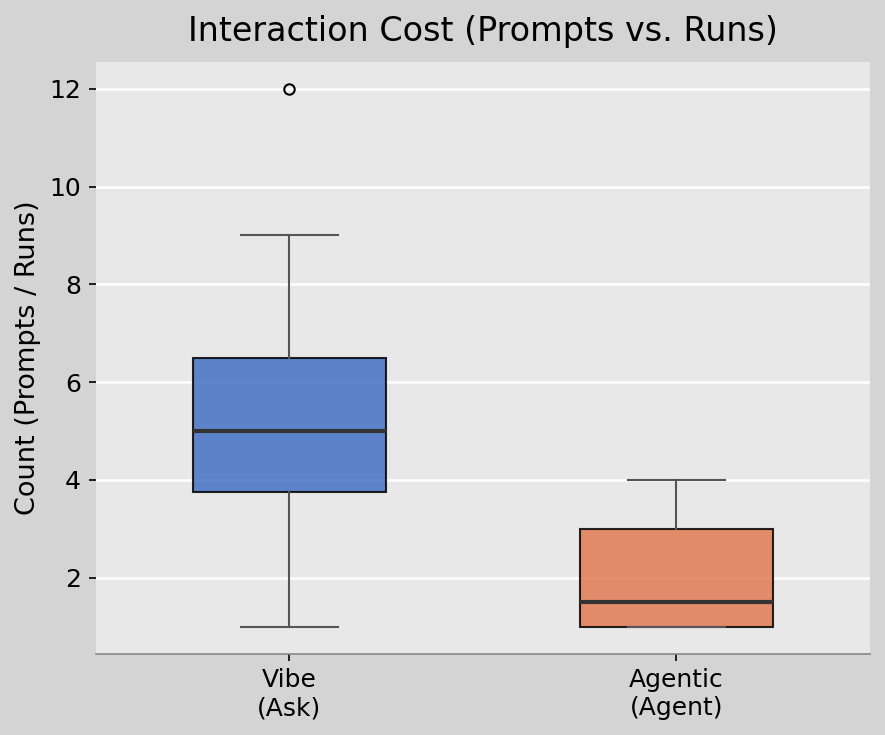
\includegraphics[width=0.6\textwidth]{figures/fig3_interaction.png}
  \caption[Interaction Cost Comparison]{Distribution of interaction costs by paradigm. Agentic Coding not only reduced the median cost but also compressed the variance in effort required.}
  \label{fig:interaction_cost}
\end{figure}

The difference was most pronounced in TG1, where Vibe Coding commonly triggered repeated prompt-and-repair cycles that each added an interaction unit and rarely converged within the time limit. Agentic Coding more often converged in a small number of multi-step runs. In TG2, Agentic Coding continued to require fewer interaction cycles, and its higher success rate (83\% vs.\ 50\%) suggests that lower interaction cost translated into more reliable task completion.

Interaction cost was positively associated with completion time across all observations (Spearman's $\rho=0.68$, $p<0.001$). This association is descriptive rather than causal; both metrics likely co-vary with task difficulty and recovery effort.

\subsection{Interruptions and Flow Breaks}

The final quantitative measure addressing RQ1 focused on interruptions, coded using the operational definition described in Section~\ref{sec:measures}. In short, interruptions capture moments where visible progress stalls due to uncertainty, tool friction, or recovery work.

Across all participants, Vibe Coding exhibited more interruptions than Agentic Coding. The median interruption count under Vibe Coding was 1 (interquartile range [0, 1]), compared to 0 under Agentic Coding (interquartile range [0, 0]; Table~\ref{tab:rq1-overview}). A Wilcoxon signed-rank test confirmed this reduction ($V=0$, $p=0.016$, rank-biserial $r=1.00$, denoting a large effect among non-tied pairs).

The qualitative character of interruptions differed by paradigm. Under Vibe Coding, interruptions typically coincided with the prompt-and-repair cycle: the pause between receiving an inadequate response and formulating the next prompt represented a break in forward progress. Under Agentic Coding, interruptions more often reflected supervision friction (monitoring an agent run, noticing drift, reviewing a larger diff before approval, or stepping in to course-correct).

Interruptions were most visible in TG1, where the more exploratory task structure created more opportunities for misalignment and recovery. In TG2, interruptions were less common overall, though the general pattern held.

% ---------------------------------------------------------

\section{Qualitative Results (RQ2: Trust, Control, and Workflow Fit)}

While the quantitative results capture efficiency and disruption outcomes, they do not fully represent how participants experienced working with the two paradigms. Research Question~2 explored how participants perceived and navigated trust, control, and workflow fit. This section combines post-session interviews and field notes.

\subsection{Coding Approach for Qualitative Data}

The qualitative analysis drew on post-session semi-structured interviews and structured observational notes anchored to specific moments in the recordings. Coding followed a deductive--inductive process: initial categories mapped to the study constructs (trust, control, workflow fit, flow), then expanded with subcodes that emerged from the data (e.g., delegation comfort, approval friction, confidence shifts). Episodes were selected based on their clarity, specificity to a concrete task moment, and recurrence across participants.

\subsection{Perceived Control and Oversight}

A consistent theme concerned the nature of control. Rather than treating control as present in one paradigm and absent in the other, participants described different control \emph{mechanisms} and different points of intervention.

Descriptively, 7 out of 12 participants leaned toward Agentic Coding as enabling better overall control, but qualified this by explaining that the control was different in nature. Agentic Coding reduced micro-decisions and shifted effort into oversight (monitoring runs, reviewing diffs, approving/rejecting actions, and intervening when the agent drifted). Several participants described this supervisory stance as efficient and empowering; others found it cognitively taxing, especially when they were unsure about what the agent was doing or why.

Vibe Coding was consistently described as supporting step-by-step steering. Participants appreciated being able to request smaller changes, inspect outputs incrementally, and correct direction early. However, when many iterations were required, the mental effort of deciding what to ask next and integrating fragmented outputs became burdensome, often embodying the prompt-and-repair cycle described in Section~\ref{sec:rq1}.

Overall, control was experienced as distributed distinctly across the task: steering in Vibe Coding versus supervision in Agentic Coding. Preferences depended on working style, confidence in reviewing larger diffs, and perceived task ambiguity.

\subsection{Trust Calibration and Verification Behavior}

Trust emerged as active and behaviorally grounded in verification strategies rather than as blanket acceptance. Across the two paradigms, participants rarely relied on the AI uncritically. Instead, they calibrated trust based on observed performance, clarity of reasoning, and, most prominently, test feedback.

Descriptively, 8 out of 12 participants reported higher confidence in Agentic Coding outcomes, often attributing this to coherent, multi-step attempts that reduced fragmentation. When an agent run produced a passing solution, participants interpreted it as evidence that the agent captured the task end-to-end.

At the same time, participants emphasized that Agentic Coding needed careful verification precisely because the AI had more autonomy. Larger multi-step changes increased the perceived risk of unintended consequences, and several participants described heightened diligence when reviewing diffs before approval (``approval anxiety''). Under Vibe Coding, confidence was frequently tied to incremental transparency: smaller changes felt easier to judge locally, even when progress was slower.

Across both models, \texttt{pytest} served as the primary verification anchor. Passing tests increased confidence; failing tests triggered strategy modifications (tightening requirements, reducing scope, or re-checking assumptions). Participants explicitly described confidence shifting after early errors or drift, leading to tighter oversight behaviors (more frequent tests, smaller requested steps, or greater constraints on what the AI should change).

\subsection{Workflow Fit and Perceived Flow}

Workflow fit captures whether a coding paradigm felt compatible with how participants prefer to work, while flow captures whether the interaction sustained focus and continued progression. These two perceptions are related but not identical: a paradigm can feel efficient yet still feel mentally disruptive.

\paragraph{Descriptive ratings.}
Figure~\ref{fig:likert_ratings} and Table~\ref{tab:rq2-likert} summarize post-task ratings (1--5). The clearest separation is on perceived efficiency: Agentic Coding scored higher ($M=4.75$, $SD=0.62$) than Vibe Coding ($M=4.00$, $SD=1.48$), and with notably less variance, meaning participants agreed more consistently that it felt efficient. Flow and focus tell a different story: the two paradigms scored almost identically (Vibe: $M=3.17$; Agentic: $M=3.08$), meaning that being faster did not translate into feeling more in the zone. Workflow fit was similarly close (Vibe: $M=3.67$; Agentic: $M=3.42$), but Agentic Coding showed much higher variability ($SD=1.62$ vs.\ $1.15$), reflecting that some participants found it a natural fit while others did not.

\begin{figure}[H]
  \centering
  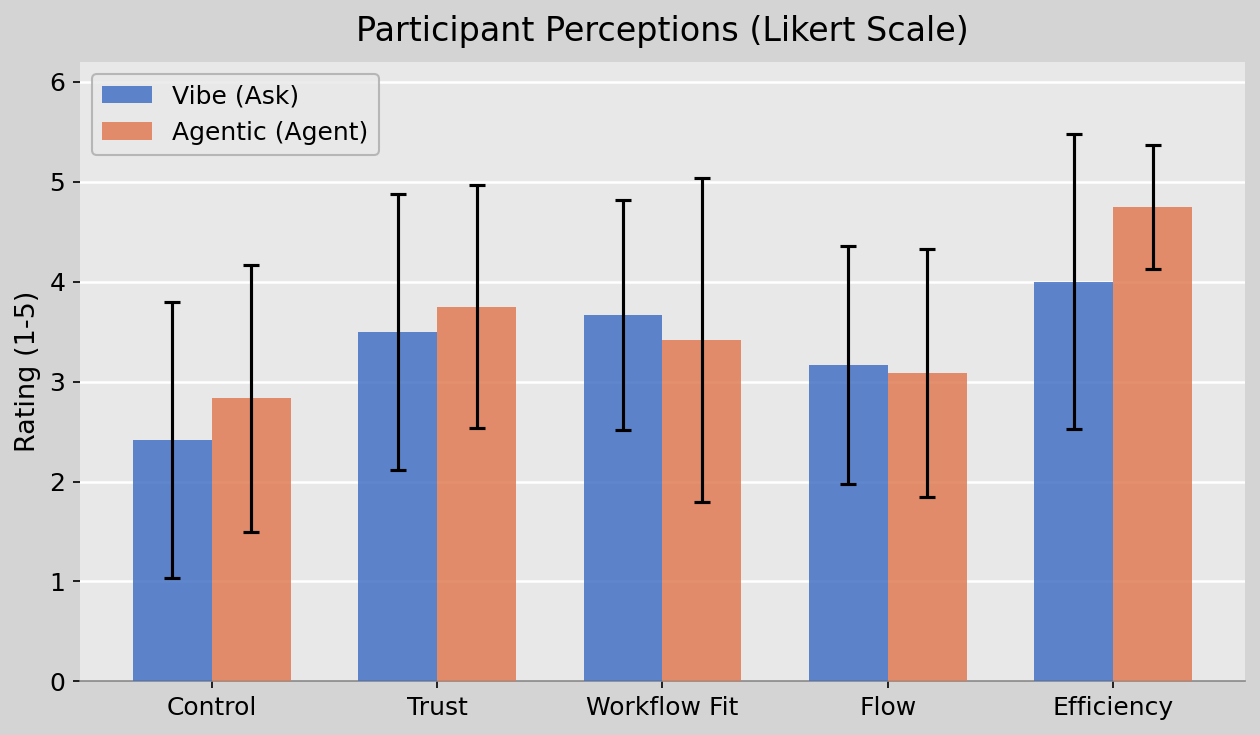
\includegraphics[width=0.9\textwidth]{figures/fig4_likert.png}
  \caption[Post-Task Likert Ratings]{Participant perceptions of the two coding paradigms (1--5). Error bars represent standard deviations. The largest separation appears for perceived efficiency; flow/focus and workflow fit show overlapping means with substantial variance.}
  \label{fig:likert_ratings}
\end{figure}

\begin{table}[H]
  \centering
  \caption[Post-task Likert ratings by paradigm]{Post-task Likert ratings (1--5) by paradigm across all task observations ($n=12$ per paradigm). Items correspond to perceived control/oversight, trust/confidence, workflow fit, flow/focus, and perceived efficiency.}
  \label{tab:rq2-likert}
  \renewcommand{\arraystretch}{1.15}
  \rowcolors{2}{gray!10}{white}
  \begin{tabular}{lcc}
    \toprule
    \rowcolor{accentblue}
    \textbf{Item (1--5)} & \textbf{Vibe Coding (mean, SD)} & \textbf{Agentic Coding (mean, SD)} \\
    \midrule
    Control / oversight & 2.42 (1.38) & 2.83 (1.34) \\
    Trust / confidence & 3.50 (1.38) & 3.75 (1.22) \\
    Workflow fit & 3.67 (1.15) & 3.42 (1.62) \\
    Flow / focus & 3.17 (1.19) & 3.08 (1.24) \\
    Perceived efficiency & 4.00 (1.48) & 4.75 (0.62) \\
    \bottomrule
  \end{tabular}
\end{table}

\paragraph{Interview synthesis.}

Interview responses help explain why efficiency was separated while flow and fit were not. In interviews, 10 out of 12 participants described Agentic Coding as more efficient overall, consistent with the quantitative reductions in completion time and interaction cost reported for RQ1. However, several participants noted that efficiency gains came with a different ``feel'' of working: instead of continuous hands-on progress, Agentic Coding sometimes shifted attention into supervision (waiting for runs, reviewing larger diffs, and intervening when drift occurred). By contrast, Vibe Coding was often described as more stepwise and transparent, supporting continuous engagement, but at the cost of conversational overhead (repeated prompt formulation and context re-establishment).

Participants also reported that workflow fit could vary by task. Agentic Coding was generally preferred for well-defined tasks where delegation felt safe, whereas Vibe Coding was sometimes preferred for more ambiguous or higher-stakes moments where tight steering felt more comfortable. These comments correspond to the higher variability in workflow-fit ratings under Agentic Coding ($SD=1.62$ vs.\ $1.15$), suggesting the paradigm fit some participants strongly while feeling mismatched for others.

\paragraph{Methodological note on Likert analysis.}

Given the ordinal nature of Likert-scale data and the small sample ($n=12$), these ratings are treated as descriptive summaries rather than as the basis for formal inferential testing. Differences between paradigms on control, trust, workflow fit, and flow are small relative to within-group variability. Perceived efficiency is the clearest separation both in mean and variance (Table~\ref{tab:rq2-likert}), which is consistent with the quantitative efficiency results reported for RQ1.

The next chapter interprets these outcomes in relation to prior literature and develops their consequences for the collaboration--delegation trade-off in AI-assisted coding. These interpretations form the foundation for the best practices proposed in Chapter~\ref{chap:conclusion}.

\chapter{Discussion}

\label{chap:discussion}

Agentic Coding was faster by every quantitative measure: it cut median completion time from 12.5 to 4.6 minutes, reduced interaction cost from a median of 5.0 prompts to 1.5 agent runs, and brought observable interruptions from a median of 1 down to 0. Yet when participants rated how the experience \emph{felt}, the two paradigms were almost indistinguishable. Perceived efficiency diverged sharply (Vibe: $M=4.00$; Agentic: $M=4.75$), but flow and workflow fit were nearly identical (flow: 3.17 vs.\ 3.08; workflow fit: 3.67 vs.\ 3.42; Table~\ref{tab:rq2-likert}). Being faster, in other words, did not make participants feel more in the zone or more naturally supported. This gap between what the stopwatch showed and what developers experienced is the central result of the study, and explaining it requires looking at the mechanisms behind the numbers rather than just the numbers themselves.

% ---------------------------------------------------------

\section{Answering RQ1: How do Vibe Coding and Agentic Coding differ in terms of developer efficiency and flow during coding activities?}

\label{sec:disc-rq1}

The efficiency advantage for Agentic Coding is clear and consistent across all four quantitative measures. Median completion time fell from 12.5 to 4.6 minutes (Wilcoxon $V=10$, $p=0.020$, rank-biserial $r=0.74$), representing a large effect. Interaction cost dropped from a median of 5.0 prompts to 1.5 agent runs ($V=0$, $p=0.0020$, $r=1.00$), and observable interruptions declined from a median of 1 to 0 ($V=0$, $p=0.016$, $r=1.00$ among non-tied pairs). Task success rates also favoured Agentic Coding (75\% versus 42\%), though the paired McNemar test did not reach significance ($p=0.289$), consistent with the limited sample size.

It is worth noting the effect of multiple comparisons. Applying a Bonferroni correction across the four RQ1 metrics yields an adjusted threshold of $\alpha_{\text{adj}} = 0.05/4 = 0.0125$. At that threshold, only interaction cost ($p=0.0020$) survives adjustment; completion time ($p=0.020$) and interruptions ($p=0.016$) both narrowly exceed it. This does not invalidate the pattern, but it means the individual $p$-values should be interpreted with caution, particularly given the sample size. The consistency of the direction across all measures is meaningful in itself.

The mechanism behind these gains is what might be called a \emph{delegation effect}: by bundling planning, editing, and test execution into integrated multi-step runs, Agentic Coding absorbed the conversational overhead that fragmented Vibe Coding workflows. Under Vibe Coding, the prompt-and-repair cycle consumed time in a way that was difficult to escape once it started, each inadequate response required a pause to reformulate, and those pauses accumulated. Agentic Coding short-circuited the cycle by letting the agent iterate internally. The strong positive association between interaction cost and completion time (Spearman $\rho=0.68$, $p<0.001$) supports this interpretation: each additional human--\gls{ai} exchange carried a measurable time cost, and Agentic Coding simply required fewer of them. This is consistent with Peng et al.'s finding that AI pair programming reduced task completion time by 55.8\% in a randomised controlled trial \parencite{peng2023copilot}, and with Sarkar et al.'s observation that higher automation levels shift developer effort from implementation to oversight \parencite{sarkar2025codewithme}.

A few alternative explanations are worth acknowledging. Despite counterbalancing, participants who completed Agentic Coding second may have accrued incidental familiarity with the repository structure; the design mitigates but cannot fully eliminate practice effects. The advantage was also most pronounced in TG1, where Vibe Coding participants frequently hit the time limit, suggesting agentic assistance may be disproportionately valuable for open-ended tasks that push participants toward their cognitive or temporal ceiling. This is discussed further in Section~\ref{sec:disc-threats}. Finally, comparing prompts to agent runs is not comparing equivalent units of effort: a single agent run can contain work equivalent to several prompts. The performance gain is real, but it reflects a reduction in discrete exchanges rather than a strictly commensurable reduction in effort.

% ---------------------------------------------------------

\section{Answering RQ2: How do developers perceive trust, control, and workflow fit when using Vibe Coding versus Agentic Coding?}

\label{sec:disc-rq2}

The subjective picture is more nuanced than the efficiency story. Ten of twelve participants rated Agentic Coding as more efficient in interviews, consistent with the quantitative results. But Likert ratings for control (Vibe: $M=2.42$; Agentic: $M=2.83$), trust (Vibe: $M=3.50$; Agentic: $M=3.75$), workflow fit (Vibe: $M=3.67$; Agentic: $M=3.42$), and flow (Vibe: $M=3.17$; Agentic: $M=3.08$) were all essentially tied, with differences small relative to within-group variability (Table~\ref{tab:rq2-likert}). Participants knew Agentic Coding was faster, but that knowledge did not translate into a consistently better felt experience.

The dominant theme in interviews was that control was not lost or gained; it was \emph{redistributed}. Vibe Coding offered fine-grained, step-by-step steering: participants chose what to ask, inspected each response, and redirected incrementally. The transparency was valued, even by participants who found the conversational overhead frustrating. Agentic Coding moved control to a higher level of abstraction: monitoring agent plans, reviewing diffs, approving or rejecting proposed changes. Seven of twelve participants preferred this supervisory stance. The remaining five were more ambivalent, describing discomfort when the agent's approach was opaque or when a diff was large enough to make careful review demanding. This finding corresponds to Barke et al.'s observation that developers adopt distinct interaction strategies with AI code generation, shifting between acceleration and exploration depending on their confidence in what the tool is doing \parencite{barke2023groundedcopilot}.

Trust interacted with autonomy in a somewhat paradoxical way. Eight of twelve participants reported higher confidence in Agentic Coding outcomes, crediting this to multi-step runs that resolved tasks in a single coherent attempt. Yet those same participants described \emph{approval anxiety}, a heightened sense of responsibility before accepting an agent's diff, precisely because each approval covered more ground and carried higher consequences than accepting a small incremental response. This pattern parallels Vaithilingam et al.'s finding that developers preferred Copilot but struggled to understand and debug its output \parencite{vaithilingam2022expectation}: preference for the tool coexisted with verification burden. Trust in AI-assisted programming is not a stable attitude; it is an ongoing calibration process anchored to verifiable outcomes in this study, primarily \texttt{pytest} results.

The most striking gap in the data is between efficiency and flow. Agentic Coding was faster across every quantitative measure, yet flow and workflow fit ratings were marginally higher under Vibe Coding (flow: 3.17 vs.\ 3.08; workflow fit: 3.67 vs.\ 3.42). Two participants explicitly preferred Vibe Coding for sustaining flow, favouring continuous hands-on involvement over the supervision intervals introduced by Agentic Coding. The higher variability in Agentic workflow-fit ratings ($SD=1.62$ vs.\ $1.15$ for Vibe) is also telling: for some participants Agentic Coding felt natural, for others it felt mismatched. This suggests that perceived efficiency and experienced flow are genuinely distinct constructs, developers can recognise that a tool makes them faster while finding its interaction rhythm less compatible with how they prefer to work. Adoption decisions are therefore unlikely to be driven by efficiency data alone.

% ---------------------------------------------------------

\section{Interaction Paradigms as a Trade-Off: Collaboration vs.\ Delegation}

\label{sec:disc-tradeoff}

The RQ1 and RQ2 findings together frame the choice between Vibe Coding and Agentic Coding as a trade-off rather than an upgrade. Agentic Coding improved every measurable efficiency dimension, lowered interaction cost, and minimised interruptions. But it also introduced friction into supervision and concentrated verification demands into fewer, higher-stakes approvals. Vibe Coding preserved transparency and incremental control at the cost of conversational overhead that fragmented workflow and slowed completion.

Task type appeared to moderate this trade-off in a predictable direction. The efficiency advantage of Agentic Coding was largest in TG1, where the open-ended data analysis tasks made the prompt-and-repair cycle particularly costly, each unsuccessful prompt consumed a larger share of the 15-minute time box (TG1 Vibe median: 15.0 min vs.\ Agentic: 6.0 min; Table~\ref{tab:rq1-by-taskgroup}). In TG2 (bug fixing), the gap narrowed (Vibe median: 8.0 min vs.\ Agentic: 3.6 min), and participants performing well-scoped repairs sometimes preferred Vibe Coding's precision. This suggests delegation benefits scale with task complexity: when the solution path is not obvious, offloading multi-step reasoning yields disproportionate gains. When the problem is well-scoped and localised, the transparency of Vibe Coding carries relatively more weight.

Experience level added a further dimension. More senior participants generally used both paradigms more deliberately, providing richer context, intervening earlier when the agent drifted, and recovering from failures faster. This is consistent with Sarkar et al.'s framework in which the benefits of higher automation depend on sufficient supervisory skill \parencite{sarkar2025codewithme}. It also suggests that the collaboration--delegation trade-off may become more navigable with experience, as developers build better mental models of when to delegate and when to steer.

% ---------------------------------------------------------

\section{Implications for Practice}

\label{sec:disc-practice}

For individual developers, the clearest implication is that paradigm selection should be deliberate rather than habitual. Agentic Coding is well-suited for tasks with clear success criteria and well-defined scope, where the agent can iterate autonomously and the developer can verify outcomes efficiently through tests. For ambiguous tasks, high-stakes changes, or situations requiring close domain reasoning throughout, Vibe Coding's incremental transparency may reduce the risk of compounding errors across multiple agent steps. Regardless of paradigm, participants who used \texttt{pytest} as a systematic checkpoint navigated both paradigms more effectively than those who relied solely on visual inspection. The tests functioned as a shared verification anchor that reduced ambiguity from each trust decision.

Agentic Coding specifically calls for practices that manage supervision friction. Scoping agent runs to a single function, test case, or bug fix makes diffs easier to review and limits the blast radius of errors. Reviewing diffs before accepting them rather than after, prevents the compounding errors that participants described as the main downside of approval anxiety. Establishing rollback points before launching a run provides a clean recovery path when the agent takes an unproductive direction. And intervening early when drift is visible is more efficient than waiting to see whether the agent self-corrects: the few Agentic interruptions in the data were predominantly supervision-related, and participants who redirected early recovered faster.

Under Vibe Coding, the analogous discipline is managing conversational overhead. Detailed initial prompts that specify requirements and constraints reduce the number of follow-up iterations and mitigate the prompt-and-repair cycle that was the primary source of time loss in this study. Constraining scope per exchange, asking for targeted changes rather than open-ended solutions, keeps each response inspectable and limits the cognitive load of integrating many partial answers. Running tests after each exchange provides the same objective anchor that helped Agentic users. And batching related requests into a single prompt reduces the interaction cost that was so strongly associated with completion time ($\rho=0.68$, $p<0.001$).

Several participants noted that the two paradigms were not mutually exclusive within a session: using Vibe Coding for exploratory or ambiguous moments and Agentic Coding for well-scoped execution could combine the benefits of both. This suggests the collaboration--delegation trade-off is not a one-time paradigm choice but a contextual judgment that can vary within a single task.

At the organisational level, onboarding and training should explicitly address the different cognitive demands of each paradigm. Developers accustomed to chat-based assistance may need guidance on effective oversight strategies before adopting agentic workflows. Code review processes may also need updating: a single multi-step agent output differs structurally from a sequence of small incremental changes, and review practices designed for the latter may not transfer well. Organisations adopting agentic tools in security-sensitive codebases should consider mandatory approval gates for destructive operations, given that unreviewed multi-step changes carry elevated risk \parencite{perry2023insecure}.

% ---------------------------------------------------------

\section{Threats to Validity and Limitations}

\label{sec:disc-threats}

\paragraph{Internal validity.} Carryover effects are the primary internal threat. Although paradigm order was counterbalanced and tasks resided in separate folders with independent starter code and tests, participants who completed Agentic Coding second may have accrued incidental familiarity with the repository structure. The within-subject design controls for individual differences but cannot fully eliminate practice effects. Additionally, the study was conducted during a period of rapid model and tool evolution; despite fixing the underlying \gls{llm} (Claude Sonnet~4.5), minor Copilot interface updates between sessions could have introduced instrumentation variability.

\paragraph{Construct validity.} The measures used to operationalise efficiency and flow are proxies rather than direct assessments. Completion time and interaction cost capture task-level performance but do not measure code quality, maintainability, or long-term comprehension. Likert items for trust, control, and flow provide a useful signal but may not capture the full dimensionality of these constructs. Interruptions were coded from observational notes, introducing observer subjectivity despite the use of structured criteria. The binary success metric (all tests passing) does not capture partial progress or the quality of intermediate reasoning.

\paragraph{External validity.} The sample of 12 participants, while sufficient for detecting large within-subject effects, limits generalisation to broader developer populations. All participants had prior Python experience and some AI tool familiarity, which may not represent developers entirely new to AI-assisted coding. Tasks were scoped to 15-minute time boxes within a single Python repository, constraining ecological validity relative to longer, multi-session development work. Findings may not transfer to other programming languages, IDEs, or AI assistance platforms with different interaction affordances.

\paragraph{Statistical conclusion validity.} The small sample limits power for small or moderate effects and precludes robust subgroup analyses by experience level or task group. As noted in Section~\ref{sec:disc-rq1}, applying a Bonferroni correction across four RQ1 metrics yields $\alpha_{\text{adj}} = 0.0125$, under which only interaction cost ($p=0.0020$) survives adjustment. Completion time ($p=0.020$) and interruptions ($p=0.016$) narrowly exceed this threshold. All reported $p$-values should be read with these considerations in mind.

% ---------------------------------------------------------

\section{Future Research Directions}

\label{sec:disc-future}

The most pressing next step is a larger-sample replication that provides statistical power for subgroup analyses by experience level and task type, and that permits formal mediation analysis of the mechanisms relating paradigm choice to efficiency gains. A crossover or between-subjects design with additional task categories such as refactoring, feature implementation, or security review would extend generalisability beyond the two task types examined here.

Future studies should likewise broaden the outcome space. Code quality and security metrics, static analysis warnings, test coverage changes, and vulnerability introduction rates \parencite{perry2023insecure, qodo2025codequality} would complement the efficiency and perception measures used here. Long-term studies tracking adoption patterns, trust calibration over time, and verification strategies as developers gain experience with agentic workflows would address something this study could not: whether the collaboration delegation trade-off shifts as the paradigm becomes familiar, and whether the approval anxiety observed here is a permanent feature of delegation or something that attenuates with practice.

% ---------------------------------------------------------

\chapter{Conclusion}

\label{chap:conclusion}

\section{Summary of Findings}

This thesis compared Vibe Coding and Agentic Coding; two AI-assisted coding paradigms, on developer efficiency, flow, and subjective experience through a within-subject experiment with 12 participants. A detailed interpretation of these results is provided in Chapter~\ref{chap:discussion}. The headline findings are as follows.

Agentic Coding was substantially faster across all quantitative measures: median task completion time fell from 12.5 to 4.6 minutes (Wilcoxon $V=10$, $p=0.020$, $r=0.74$), interaction cost dropped from a median of 5.0 prompts to 1.5 agent runs ($p=0.0020$, $r=1.00$), and observable interruptions declined from a median of 1 to 0 ($p=0.016$). Task success rates favoured Agentic Coding descriptively (75\% versus 42\%), though the difference did not reach significance at the sample size used ($p=0.289$). Under a Bonferroni correction for four simultaneous tests ($\alpha_{\text{adj}}=0.0125$), only the interaction cost result survives; completion time and interruptions narrowly exceed the adjusted threshold.

Subjective experience did not mirror these efficiency gains. Ten of twelve participants rated Agentic Coding as more efficient in interviews, yet Likert ratings for flow (3.17 vs.\ 3.08), workflow fit (3.67 vs.\ 3.42), control (2.42 vs.\ 2.83), and trust (3.50 vs.\ 3.75) were all essentially tied between paradigms. Control was redistributed rather than gained or lost: Vibe Coding offered incremental steering while Agentic Coding moved to supervisory oversight. Trust in both paradigms was verification-driven and anchored primarily to \texttt{pytest} outcomes. The higher variability in Agentic workflow-fit ratings ($SD=1.62$ vs.\ $1.15$) reflects genuine individual differences in how well delegation matched each participant's working style.

The core finding is that paradigm choice is a genuine trade-off, not an upgrade. Efficiency and experienced flow can diverge. Paradigm selection should depend on task characteristics, verification infrastructure, and working style not on a blanket preference for automation.

\pagebreak

% ---------------------------------------------------------

\section{Best Practices for Using the Two AI Coding Paradigms}

Based on the empirical findings and qualitative patterns observed during sessions, the following concrete practices emerged for each paradigm.

\paragraph{Vibe Coding.}

\begin{enumerate}

  \item \textbf{Front-load context in prompts.} Detailed initial prompts that specify requirements, constraints, and expected behaviour reduce the number of follow-up iterations and mitigate the prompt-and-repair cycle that was the primary source of time loss in this study (median interaction cost: 5.0 prompts vs.\ 1.5 agent runs; Section~\ref{sec:rq1}).

  \item \textbf{Constrain scope per interaction.} Requesting small, targeted changes rather than open-ended solutions keeps each response inspectable and limits the cognitive load of integrating many partial answers. Participants who valued this granularity described it as the core advantage of Vibe Coding's steering model (Section~\ref{sec:disc-rq2}).

  \item \textbf{Use tests as checkpoints.} Running the test suite after each exchange provides an objective anchor for deciding whether to continue in the current direction or change course. Across both paradigms, \texttt{pytest} outcomes served as the dominant trust-calibration mechanism (Section~\ref{sec:disc-rq2}); under Vibe Coding specifically, they helped prevent drift across many iterations.

  \item \textbf{Batch related requests.} When several changes address the same function or module, combining them in a single prompt avoids redundant context-setting and preserves momentum. The strong association between interaction cost and completion time (Spearman's $\rho=0.68$, $p<0.001$; Section~\ref{sec:rq1}) suggests that each additional exchange carries a measurable time penalty.

\end{enumerate}

\paragraph{Agentic Coding.}

\begin{enumerate}

  \item \textbf{Scope agent runs to well-defined subtasks.} Narrowing the agent's objective to a single function, test case, or bug fix makes diffs easier to review and limits the blast radius of errors. This directly addresses the oversight burden that participants identified as Agentic Coding's main friction point (Section~\ref{sec:disc-tradeoff}).

  \item \textbf{Review diffs before approval.} Because a single agent run can span multiple files and dozens of lines, inspecting proposed changes \emph{before} accepting them prevents compounding errors that are costly to unwind. The approval anxiety reported by participants (Section~\ref{sec:disc-rq2}) stemmed precisely from situations where diffs were accepted without thorough review.

  \item \textbf{Establish rollback points.} Committing or stashing the working state before launching an agent run provides a safe return path if the run produces unintended side effects. Agentic Coding failures in TG1 were frequently associated with early missteps that lacked a clean recovery path (Section~\ref{sec:rq1}).

  \item \textbf{Act early on drift.} When the agent pursues an unproductive direction, stopping the run and re-scoping the instruction is more efficient than allowing it to compound errors across further steps. Participants who intervened promptly recovered faster than those who waited (Section~\ref{sec:rq1}).

\end{enumerate}

These practices are not mutually exclusive. Several participants noted that alternating between paradigms within a session using Vibe Coding for exploratory reasoning and Agentic Coding for well-scoped execution could combine the advantages of both approaches.

% ---------------------------------------------------------

\section{Contributions and Outlook}

This thesis makes four contributions. First, it provides, to the best of the author's knowledge, one of the earliest controlled empirical comparisons of conversational and agentic AI-assisted coding paradigms within a single IDE, using a within-subject design that isolates the paradigm variable from tool and model confounds. Second, it delivers a paired dataset of 24 task-level observations, session recordings, and qualitative interview data that can support secondary analysis and replication. Third, it offers quantitative evidence that agentic assistance substantially reduces completion time, interaction cost, and interruptions while also documenting the supervision friction and trust dynamics that accompany delegation. Fourth, it translates these findings into implementable best practices for developers and organisations adopting AI coding tools.

The near-term outlook for agentic coding is one of rapid adoption alongside open questions. As AI models and tool integrations continue to mature, the efficiency advantages documented here will likely grow, particularly for tasks with well-defined success criteria. What remains unclear is how developers will calibrate trust and oversight over longer time horizons, whether agentic workflows will cause systematic code quality or security risks that short-term studies cannot detect \parencite{perry2023insecure, qodo2025codequality}, and how team-level review processes will adapt to the larger, more coherent changesets that agentic tools produce. Answering these questions will require longitudinal field studies and expanded outcome measures that go beyond efficiency to encompass maintainability, security, and developer skill development.

% ---------------------------------------------------------

\section{Learnings and Reflections}

Beyond the formal contributions of this thesis, the process of completing it produced a set of personal learnings worth briefly acknowledging. From a practical standpoint, this thesis required acquiring several capabilities from scratch. Prior to beginning, \LaTeX{} was unfamiliar territory, and formal research methodology, experimental design, statistical testing, qualitative coding had not previously been applied in a structured scholarly context. These competencies were built iteratively throughout the writing process itself, meaning the thesis served simultaneously as subject and training ground.

Keeping pace with the subject matter presented its own ongoing challenge. AI developments move faster than most academic domains, and maintaining an accurate picture of the state of the field required active, continuous engagement throughout the entire duration of the project: tracking model releases, reading preprints, and revising framing as the landscape shifted. This is reflected in the thesis itself, which incorporates developments from early 2026 an unusual situation for a thesis still in progress at the time.

The observational sessions, however, produced the most genuinely surprising insights. Observing twelve developers work with the same tools on the same tasks revealed a degree of individual variation that was not anticipated. What stood out most was the behaviour of more senior participants. The intuitive expectation going in was that experienced engineers would carry some resistance or doubt toward AI-generated output. Instead, several senior participants evaluated the agent's contributions on their merits, and in more than one instance remarked that the output was of a quality that would have been difficult to produce themselves in the same timeframe. This corresponded with an emerging pattern in the literature suggesting that assumptions about generational resistance to AI tooling are already being challenged in practice.

Finally, observing real developers navigate these trade-offs brought the best practices documented in this thesis out of the abstract and into something more concrete and personally applicable. Recognising firsthand when delegation genuinely serves a task and when retaining granular control is the better choice is a lesson that goes beyond the research findings into everyday development practice.


\printbibliography[heading=bibintoc]
\cleardoublepage
\phantomsection

\cleardoublepage
\phantomsection
\addcontentsline{toc}{chapter}{Appendix}
\appendix
\pagestyle{plain}
\begin{appendices}
\appendix
\chapter{Study Tasks}

% =========================
% Task Group 1
% =========================
\section[Github Repo Explanation]{COPILOT-VIBE-AGENTIC-CODING-STUDY}
\label{app:repo}
\begin{lstlisting}[language=]
# Copilot Vibe Agentic Coding Study

This repository contains coding tasks for a study comparing two modes of GitHub Copilot: Vibe Coding (Ask Mode) and Agentic Coding (Agent Mode).

## Participant Groups

- **Group 1 (GAIA-inspired Tasks):** Data analysis and CSV processing tasks using Python's standard library.
  - Assigned tasks: `task_group_1/task_1a/` and `task_group_1/task_1b/`.
- **Group 2 (SWE-inspired Tasks):** Bug-fixing tasks in Python configuration parsers.
  - Assigned tasks: `task_group_2/task_2a/` and `task_group_2/task_2b/`.

You will be assigned to one group based on the study design.

## Repository Contents

- `task_group_1/`: Data Analysis Tasks (Group 1)
  - `task_1a/`: **GAIA-a - Invasive Species Research**: Analyze USGS CSV data to find unique ZIP codes where clownfish (from *Finding Nemo*) was observed as nonnative before 2020. Filter by species name, data source, and observation year. Return sorted list of 5-digit ZIP codes.
  - `task_1b/`: **GAIA-b - British Museum Mollusk Shell & Bead Age**: Analyze research articles CSV to find the minimum age of beads made from a specific mollusk species linked to British Museum object "2012,5015.17". Filter by journal (Science Advances), publication year (2021), and return minimum age in thousands of years.

- `task_group_2/`: Software Engineering Bug-Fixing Tasks (Group 2)
  - `task_2a/`: **CSV Parser Case Sensitivity Bug**: Fix a CSV configuration parser that crashes on lowercase commands. The parser reads special command lines (like `#SKIP` or `#DELIMITER`) but only recognizes UPPERCASE versions. Make command parsing case-insensitive so `#skip`, `#Skip`, and `#SKIP` all work.
  - `task_2b/`: **JSON Config Validation Bug**: Fix a configuration validator that fails to handle boolean values represented as strings. Add support for converting string representations (`"true"`, `"false"`, `"1"`, `"0"`) to proper boolean types, similar to existing int/float conversion.

- Each task folder has its own README with detailed instructions, starter code, tests, and data files (for Group 1).

## Experiment Process (Step-by-Step)

The study takes 60 minutes total. Follow these steps in order:

1. **Phase 1: Onboarding & Consent (10 minutes)**
   - Arrive and review the study procedure.
   - Sign consent form.
   - Complete a background survey (experience with AI tools, programming).

2. **Phase 2: Task 1 Coding Session (15 minutes)**
   - The researcher assigns you a Copilot mode (Vibe or Agentic) for this task.
   - Navigate to your assigned task folder (based on your group).
   - Read the task README and implement the code using the assigned mode.
   - Screen recording and time tracking will occur.

3. **Phase 3: Post-Task Survey 1 (5 minutes)**
   - Complete a short survey rating the mode you just used.
   - Sample questions (Likert scale: 1-5, Strongly Disagree to Strongly Agree):
     - "I trusted the AI suggestions."
     - "The mode aligned with my workflow."
     - "I felt in control of the coding process."
   - Write a brief reflection (e.g., "What was frustrating?").

4. **Phase 4: Task 2 Coding Session (15 minutes)**
   - Switch to the other Copilot mode.
   - Work on the second task in your group.
   - Screen recording continues.

5. **Phase 5: Post-Task Survey 2 (5 minutes)**
   - Rate the second mode with similar Likert questions.
   - Write a brief reflection.

6. **Phase 6: Comparative Interview (10 minutes)**
   - Discuss your experiences with both modes.
   - Answer comparative questions (e.g., "Which mode was more efficient?").

**Important:** Stick to the time limits. Do not switch modes mid-task. The researcher will guide you through each phase.

\end{lstlisting}
\section{Task Group 1}
Task materials are provided in Appendix~\ref{app:tg1a-code} and Appendix~\ref{app:tg1b-code}.

\begin{figure}[ht]
\setlength{\fboxsep}{5pt}
\centering
\begin{minipage}[t]{1\textwidth}
\fbox{%
\parbox{\textwidth}{\footnotesize
\textbf{Task Group 1 (TG1): Data analysis tasks}\par\medskip
\texttt{task\_group\_1/}\\
\texttt{├─ task\_1a/}\\
\texttt{│\ \ ├─ README.md}\\
\texttt{│\ \ ├─ data/ \ \ \ \ \ (CSV)}\\
\texttt{│\ \ ├─ src/ \ \ \ \ \ (solution.py)}\\
\texttt{│\ \ └─ tests/ \ \ (test\_solution.py)}\\
\texttt{└─ task\_1b/}\\
\texttt{\hspace*{1.6em}├─ README.md}\\
\texttt{\hspace*{1.6em}├─ data/ \ \ \ \ \ (CSV)}\\
\texttt{\hspace*{1.6em}├─ src/ \ \ \ \ \ (solution.py)}\\
\texttt{\hspace*{1.6em}└─ tests/ \ \ (test\_solution.py)}\\
}}
\end{minipage}
\end{figure}

\subsection{Task 1a}
\label{app:tg1a-code}
\begin{lstlisting}[language=]
# task_group_1/task_1a/README.md
# Task Group 1: Data Analysis Tasks

## Steps to Complete Task Group 1

1. Install Python
   - Download and install Python 3.6+ from [python.org](https://www.python.org/downloads/)
   - Verify installation: `python --version`
   - Ensure pip is available: `pip --version`
     - If not, install via `python get-pip.py` (download from bootstrap.pypa.io) or `python -m ensurepip --upgrade`

2. Set up the project environment
   - Navigate to the task directory: `cd task_group_1/task_1a/`
   - (Optional) Create a virtual environment for isolation: `python -m venv venv` then activate it
   - Install testing dependencies: `python -m pip install pytest` (use `python -m pip` instead of `pip` directly, as `pip` may not be in PATH)
   - *Note for macOS/Apple users: If you encounter issues, you may need to install Python via Homebrew (`brew install python3`) or use `python3` instead of `python`*

3. Implement the solution
   - Read `task_1a/README.md` for details
   - Edit `task_1a/src/solution.py` to implement the required function

4. Run and validate the solution
   - Execute tests: `python -m pytest` (from `task_1a/` directory)
   - Ensure all tests pass

# GAIA-a – Invasive Species Research (Data Analysis Task)

## Task Overview

Analyze a CSV of USGS invasive species records for a pet fish from *Finding Nemo*. Find all unique 5-digit ZIP codes where this fish was observed as nonnative before 2020. Do not use web access or external APIs.

## Files and Structure

```
.
├─ README.md                # This file
├─ data/
│  └─ usgs_nemo_observations.csv
├─ src/
│  └─ solution.py           # Implement your solution here
└─ tests/
   └─ test_solution.py      # Automated tests
```

### data/usgs_nemo_observations.csv

CSV with columns: `species_common_name`, `data_source`, `observation_year`, `zip_code`, etc. Inspect header for exact names.

## What You Need to Implement

Implement in `src/solution.py`:

```python
from typing import List

def find_nonnative_zip_codes(csv_path: str = "data/usgs_nemo_observations.csv") -> List[str]:
    """
    Return unique 5-digit ZIP codes where the Nemo fish (clownfish) was observed as nonnative by USGS before 2020.
    Filter: data_source == "USGS", observation_year < 2020, species contains "clownfish" (case-insensitive).
    Return sorted list of strings.
    """
    ...
```

## Input / Output

- **Input:** CSV path (default: "data/usgs_nemo_observations.csv")
- **Output:** List[str] of unique ZIP codes, sorted ascending.

Example: ["33040", "60601", "96701", "96706", "96734"]

## Constraints

- Python 3, standard library only.
- Do not modify CSV or test files.

## Evaluation

Tests check correct filtering, unique/sorted ZIP codes, and match expected results.

## Hints

- Use `csv` module.
- Lowercase for species matching.
- ZIP codes as strings to preserve leading zeros.
- Use `set` for uniqueness, then sort.

---

# Görev Grubu 1: Veri Analizi Görevleri

## Görev Grubu 1'i Tamamlama Adımları

1. Python'u Yükleyin
   - Python 3.6+ sürümünü [python.org](https://www.python.org/downloads/) adresinden indirip yükleyin
   - Kurulumu doğrulayın: `python --version`
   - pip'in mevcut olduğundan emin olun: `pip --version`
     - Değilse, `python get-pip.py` (bootstrap.pypa.io'dan indirin) veya `python -m ensurepip --upgrade` ile yükleyin

2. Proje ortamını kurun
   - Görev dizinine gidin: `cd task_group_1/task_1a/`
   - (İsteğe bağlı) İzolasyon için sanal ortam oluşturun: `python -m venv venv` ardından aktif edin
   - Test bağımlılıklarını yükleyin: `python -m pip install pytest` (PATH'te olmayabileceğinden `pip` yerine `python -m pip` kullanın)

3. Çözümü uygulayın
   - Detaylar için `task_1a/README.md` dosyasını okuyun
   - Gerekli fonksiyonu uygulamak için `task_1a/src/solution.py` dosyasını düzenleyin

4. Çözümü çalıştırın ve doğrulayın
   - Testleri çalıştırın: `python -m pytest` (`task_1a/` dizininden)
   - Tüm testlerin geçtiğinden emin olun

# GAIA-a – İstilacı Tür Araştırması (Veri Analizi Görevi)

## Görev Özeti

*Finding Nemo* filminden bir evcil balık için USGS istilacı tür kayıtlarının bulunduğu bir CSV dosyasını analiz edin. Bu balığın 2020'den önce yerli olmayan tür olarak gözlemlendiği tüm benzersiz 5 haneli posta kodlarını bulun. Web erişimi veya harici API kullanmayın.

## Dosyalar ve Yapı

```
.
├─ README.md                # Bu dosya
├─ data/
│  └─ usgs_nemo_observations.csv
├─ src/
│  └─ solution.py           # Çözümünüzü buraya uygulayın
└─ tests/
   └─ test_solution.py      # Otomatik testler
```

### data/usgs_nemo_observations.csv

Sütunları içeren CSV: `species_common_name`, `data_source`, `observation_year`, `zip_code`, vb. Tam isimler için başlığı inceleyin.

## Uygulamanız Gerekenler

`src/solution.py` dosyasında uygulayın:

```python
from typing import List

def find_nonnative_zip_codes(csv_path: str = "data/usgs_nemo_observations.csv") -> List[str]:
    """
    Nemo balığının (palyaço balığı) 2020'den önce USGS tarafından yerli olmayan tür olarak 
    gözlemlendiği benzersiz 5 haneli posta kodlarını döndürün.
    Filtre: data_source == "USGS", observation_year < 2020, tür adında "clownfish" içerir (büyük/küçük harf duyarsız).
    Sıralanmış string listesi döndürün.
    """
    ...
```

## Girdi / Çıktı

- **Girdi:** CSV dosya yolu (varsayılan: "data/usgs_nemo_observations.csv")
- **Çıktı:** Artan sırada sıralanmış benzersiz posta kodlarının List[str] listesi.

Örnek: ["33040", "60601", "96701", "96706", "96734"]

## Kısıtlamalar

- Python 3, sadece standart kütüphane.
- CSV veya test dosyalarını değiştirmeyin.

## Değerlendirme

Testler doğru filtreleme, benzersiz/sıralı posta kodları ve beklenen sonuçlarla eşleşmeyi kontrol eder.

## İpuçları

- `csv` modülünü kullanın.
- Tür eşleştirmesi için küçük harf kullanın.
- Başta sıfırları korumak için posta kodlarını string olarak tutun.
- Benzersizlik için `set` kullanın, sonra sıralayın.
\end{lstlisting}
\begin{lstlisting}[language=]
# task_group_1/task_1a/data/usgs_nemo_observations.csv

species_common_name,data_source,observation_year,zip_code,notes
Ocellaris Clownfish,USGS,2015,33040,Recorded in residential canal
Ocellaris Clownfish,USGS,2016,96706,Reef-adjacent sighting
Ocellaris Clownfish,USGS,2018,96706,Duplicate location entry
Ocellaris Clownfish,USGS,2012,33040,Earlier sighting
Ocellaris Clownfish,USGS,2017,96701,Confirmed pet-release
Ocellaris Clownfish,USGS,2021,96701,Post-2020 (should not count)
Ocellaris Clownfish,AquariumTradeDB,2015,96706,Non-USGS source (ignore)
Ocellaris Clownfish,USGS,2019,96734,Local lagoon observation
Ocellaris Clownfish,USGS,2020,96734,Year is 2020 (should not count)
Ocellaris Clownfish,USGS,2014,60601,Isolated aquarium-release report
\end{lstlisting}
\begin{lstlisting}[language=Python]
# task_group_1/task_1a/src/solution.py

from typing import List

def find_nonnative_zip_codes(csv_path: str = "data/usgs_nemo_observations.csv") -> List[str]:
    """
    Return unique 5-digit ZIP codes where the Nemo fish (clownfish) was observed as nonnative by USGS before 2020.
    Filter: data_source == "USGS", observation_year < 2020, species contains "clownfish" (case-insensitive).
    Return sorted list of strings.
    """
    ...
\end{lstlisting}
\begin{lstlisting}[language=Python]
# task_group_1/task_1a/tests/test_solution.py

import pytest
from src.solution import find_nonnative_zip_codes

def test_find_nonnative_zip_codes():
    result = find_nonnative_zip_codes()
    expected = ["33040", "60601", "96701", "96706", "96734"]
    assert result == expected, f"Expected {expected}, got {result}"

def test_find_nonnative_zip_codes_with_custom_path():
    result = find_nonnative_zip_codes("data/usgs_nemo_observations.csv")
    expected = ["33040", "60601", "96701", "96706", "96734"]
    assert result == expected
\end{lstlisting}

\subsection{Task 1b}
\label{app:tg1b-code}

\begin{lstlisting}[language=]
# task_group_1/task_1b/README.MD
# Task Group 1: Data Analysis Tasks

## Steps to Complete Task Group 1

1. Install Python
   - Download and install Python 3.6+ from [python.org](https://www.python.org/downloads/)
   - Verify installation: `python --version`
   - Ensure pip is available: `pip --version`
     - If not, install via `python get-pip.py` (download from bootstrap.pypa.io) or `python -m ensurepip --upgrade`

2. Set up the project environment
   - Navigate to the task directory: `cd task_group_1/task_1b/`
   - (Optional) Create a virtual environment for isolation: `python -m venv venv` then activate it
   - Install testing dependencies: `python -m pip install pytest` (use `python -m pip` instead of `pip` directly, as `pip` may not be in PATH)
   - *Note for macOS/Apple users: If you encounter issues, you may need to install Python via Homebrew (`brew install python3`) or use `python3` instead of `python`*

3. Implement the solution
   - Read the task description below
   - Edit `src/solution.py` to implement the required function

4. Run and validate the solution
   - Execute tests: `python -m pytest` (from `task_1b/` directory)
   - Ensure all tests pass




Below is the deeper explanation of 
# GAIA-b — British Museum Mollusk Shell & Bead Age (Data Analysis Task)

## Task Overview

Analyze a CSV of mollusk bead research articles to find the minimum age of beads made from a specific species' shells. The species is linked to a British Museum object.

Find the minimum "at least" age (in thousands of years) from 2021 *Science Advances* articles about that species.

## Files and Structure

```
.
├─ README.md                # This file
├─ data/
│  └─ mollusk_bead_articles.csv
├─ src/
│  └─ solution.py           # Implement your solution here
└─ tests/
   └─ test_solution.py      # Automated tests
```

### data/mollusk_bead_articles.csv

CSV with columns: `museum_number`, `accepted_species_name`, `journal`, `publication_year`, `min_age_thousand_years_at_least`, etc.

## What You Need to Implement

Implement in `src/solution.py`:

```python
def find_min_bead_age(csv_path: str = "data/mollusk_bead_articles.csv") -> int:
    """
    Find the minimum 'at least' age (in thousands of years) of beads made from the mollusk species
    linked to British Museum object '2012,5015.17', as reported in 2021 Science Advances articles.
    """
    ...
```

## Input / Output

- **Input:** CSV path (default: "data/mollusk_bead_articles.csv")
- **Output:** Integer of the minimum age.

## Constraints

- Python 3, standard library only.
- Do not modify CSV or test files.

## Evaluation

Tests check the correct minimum age is returned.

## Hints

- Use `csv` module.
- Find species from museum_number "2012,5015.17".
- Filter by species, journal "Science Advances", year 2021.
- Find min of `min_age_thousand_years_at_least`.

---

# Görev Grubu 1: Veri Analizi Görevleri

## Görev Grubu 1'i Tamamlama Adımları

1. Python'u Yükleyin
   - Python 3.6+ sürümünü [python.org](https://www.python.org/downloads/) adresinden indirip yükleyin
   - Kurulumu doğrulayın: `python --version`
   - pip'in mevcut olduğundan emin olun: `pip --version`
     - Değilse, `python get-pip.py` (bootstrap.pypa.io'dan indirin) veya `python -m ensurepip --upgrade` ile yükleyin

2. Proje ortamını kurun
   - Görev dizinine gidin: `cd task_group_1/task_1b/`
   - (İsteğe bağlı) İzolasyon için sanal ortam oluşturun: `python -m venv venv` ardından aktif edin
   - Test bağımlılıklarını yükleyin: `python -m pip install pytest` (PATH'te olmayabileceğinden `pip` yerine `python -m pip` kullanın)

3. Çözümü uygulayın
   - Aşağıdaki görev açıklamasını okuyun
   - Gerekli fonksiyonu uygulamak için `src/solution.py` dosyasını düzenleyin

4. Çözümü çalıştırın ve doğrulayın
   - Testleri çalıştırın: `python -m pytest` (`task_1b/` dizininden)
   - Tüm testlerin geçtiğinden emin olun

# GAIA-b — British Museum Mollusk Kabuğu & Boncuk Yaşı (Veri Analizi Görevi)

## Görev Özeti

Belirli bir türün kabuklarından yapılmış boncukların minimum yaşını bulmak için mollusk boncuk araştırma makalelerinin bulunduğu bir CSV dosyasını analiz edin. Tür, bir British Museum nesnesine bağlıdır.

British Museum "2012,5015.17" nesnesiyle ilişkili türle ilgili 2021 *Science Advances* makalelerinden "en az" minimum yaşı (bin yıl cinsinden) bulun.

## Dosyalar ve Yapı

```
.
├─ README.md                # Bu dosya
├─ data/
│  └─ mollusk_bead_articles.csv
├─ src/
│  └─ solution.py           # Çözümünüzü buraya uygulayın
└─ tests/
   └─ test_solution.py      # Otomatik testler
```

### data/mollusk_bead_articles.csv

Sütunları içeren CSV: `museum_number`, `accepted_species_name`, `journal`, `publication_year`, `min_age_thousand_years_at_least`, vb.

## Uygulamanız Gerekenler

`src/solution.py` dosyasında uygulayın:

```python
def find_min_bead_age(csv_path: str = "data/mollusk_bead_articles.csv") -> int:
    """
    British Museum nesnesi '2012,5015.17' ile ilişkili mollusk türünden yapılmış boncukların
    2021 Science Advances makalelerinde bildirilen minimum 'en az' yaşını (bin yıl cinsinden) bulun.
    """
    ...
```

## Girdi / Çıktı

- **Girdi:** CSV dosya yolu (varsayılan: "data/mollusk_bead_articles.csv")
- **Çıktı:** Minimum yaşın tam sayı değeri.

## Kısıtlamalar

- Python 3, sadece standart kütüphane.
- CSV veya test dosyalarını değiştirmeyin.

## Değerlendirme

Testler doğru minimum yaşın döndürüldüğünü kontrol eder.

## İpuçları

- `csv` modülünü kullanın.
- museum_number "2012,5015.17" den türü bulun.
- Türe, "Science Advances" dergisine ve 2021 yılına göre filtreleyin.
- `min_age_thousand_years_at_least` değerinin minimumunu bulun.
\end{lstlisting}
\begin{lstlisting}[language=]
# task_group_1/task_1b/data/mollusk_bead_articles.csv

museum_number,accepted_species_name,journal,publication_year,min_age_thousand_years_at_least,notes
2012,5015.17,Nassarius gibbosulus,,,
,Nassarius gibbosulus,Science Advances,2021,100,Bead age study 1
,Nassarius gibbosulus,Science Advances,2021,120,Bead age study 2
,Nassarius gibbosulus,Science Advances,2021,90,Bead age study 3
,Nassarius gibbosulus,Nature,2021,80,Different journal
,Nassarius gibbosulus,Science Advances,2020,95,Wrong year
,Other species,Science Advances,2021,50,Different species
\end{lstlisting}
\begin{lstlisting}[language=Python]
# task_group_1/task_1b/src/solution.py

from typing import List

def find_min_bead_age(csv_path: str = "data/mollusk_bead_articles.csv") -> int:
    """
    Find the minimum 'at least' age (in thousands of years) of beads made from the mollusk species
    linked to British Museum object '2012,5015.17', as reported in 2021 Science Advances articles.
    """
    ...
\end{lstlisting}
\begin{lstlisting}[language=Python]
# task_group_1/task_1b/tests/test_solution.py

import pytest
from src.solution import find_min_bead_age

def test_find_min_bead_age():
    result = find_min_bead_age()
    expected = 90
    assert result == expected, f"Expected {expected}, got {result}"

def test_find_min_bead_age_with_custom_path():
    result = find_min_bead_age("data/mollusk_bead_articles.csv")
    expected = 90
    assert result == expected
\end{lstlisting}

% =========================
% Task Group 2
% =========================
\section{Task Group 2}
Task materials are provided in Appendix~\ref{app:tg2a-code} and Appendix~\ref{app:tg2b-code}.
\begin{figure}[ht]
\setlength{\fboxsep}{5pt}
\centering
\begin{minipage}[t]{1\textwidth}
\fbox{%
\parbox{\textwidth}{\footnotesize
\textbf{Task Group 2 (TG2): Bug-fixing tasks}\par\medskip
\texttt{task\_group\_2/}\\
\texttt{├─ task\_2a/}\\
\texttt{│\ \ ├─ README.md}\\
\texttt{│\ \ ├─ src/ \ \ \ \ \ (solution.py, demo.py)}\\
\texttt{│\ \ └─ tests/ \ \ (test\_solution.py)}\\
\texttt{└─ task\_2b/}\\
\texttt{\hspace*{1.6em}├─ README.md}\\
\texttt{\hspace*{1.6em}├─ src/ \ \ \ \ \ (solution.py, demo.py)}\\
\texttt{\hspace*{1.6em}└─ tests/ \ \ (test\_solution.py)}\\
\texttt{\hspace*{1.6em}}\\
\texttt{\hspace*{1.6em}}\\
}}
\end{minipage}
\end{figure}

\subsection{Task 2a}
\label{app:tg2a-code}
\begin{lstlisting}[language=]
# task_group_2/task_2a/README.MD
# Task Group 2: SWE-inspired Tasks

## Steps to Complete Task Group 2

1. Install Python
   - Download and install Python 3.6+ from [python.org](https://www.python.org/downloads/)
   - Verify installation: `python --version`
   - Ensure pip is available: `pip --version`
     - If not, install via `python get-pip.py` (download from bootstrap.pypa.io) or `python -m ensurepip --upgrade`

2. Set up the project environment
   - Navigate to the task directory: `cd task_group_2/task_2a/`
   - (Optional) Create a virtual environment for isolation: `python -m venv venv` then activate it
   - Install dependencies: `python -m pip install matplotlib numpy`
   - *Note for macOS/Apple users: If you encounter issues, you may need to install Python via Homebrew (`brew install python3`) or use `python3` instead of `python`. For matplotlib on macOS, you might also need to install with `brew install python-tk` for GUI support*

3. Implement the solution
   - Read the task description below
   - Edit `src/solution.py` to implement the required functions

4. Run and validate the solution
   - Execute tests: `python -m pytest` (from `task_2a/` directory)
   - Or run the demo: `python src/demo.py`

---

# Task 2a: Fix CSV Parser Case Sensitivity Bug

## Objective

**This is a bug-fixing task.** A CSV configuration parser was implemented to read special commands from CSV files, but it incorrectly assumes all commands must be UPPERCASE. Real users create files by hand and use lowercase commands, causing the parser to crash.

## Issue Description

The `parse_csv_with_commands()` function reads CSV files that can contain special command lines starting with `#` (like `#SKIP 2` or `#DELIMITER tab`). However, the parser only recognizes UPPERCASE commands and crashes on lowercase ones.

### Example of the Problem

This file crashes:
```
#skip 2
#delimiter tab
Name	Value	Error
Alice	1.5	0.1
```

But this works fine:
```
#SKIP 2
#DELIMITER tab
Name	Value	Error
Alice	1.5	0.1
```

Since users create these files by hand, the parser should be case-insensitive like other tools.

## How to Reproduce

```python
from solution import parse_csv_with_commands

# This crashes with "Unrecognized command: #skip 2"
data = """#skip 2
#delimiter tab
Name	Value
Alice	1.5
Bob	2.3"""

result = parse_csv_with_commands(data)
```

## Your Task

**Fix the bug in `src/solution.py`** to make command parsing case-insensitive.

The parser currently checks commands like:
```python
if line.startswith('#SKIP'):
    # handle skip
elif line.startswith('#DELIMITER'):
    # handle delimiter
```

**Hint**: Convert the line to uppercase before checking, or use case-insensitive comparison.

### Expected Behavior

After fixing:
- `#SKIP 2`, `#skip 2`, `#Skip 2` should all work
- `#DELIMITER tab`, `#delimiter tab`, `#Delimiter tab` should all work
- The parser should handle mixed case in command names

## Files Structure

```
.
├─ README.md                # This file
├─ src/
│  ├─ solution.py           # FIX THE BUG HERE
│  └─ demo.py               # Demo script
└─ tests/
   └─ test_solution.py      # Tests
```

## Debugging Tips

1. Run the tests: `python -m pytest tests/ -v`
2. Try parsing files with lowercase commands
3. Check where command recognition happens
4. Use `.upper()` or `.lower()` for case-insensitive comparison

## Constraints

- Python 3, use matplotlib and numpy.
- Do not modify test files.

## Hints

- Use `matplotlib.animation.FuncAnimation` for animations.
- Implement easing functions for smooth transitions.
- Consider using numpy for interpolation between data states.

---

# Görev Grubu 2: Yazılım Mühendisliği Görevleri

## Görev Grubu 2'yi Tamamlama Adımları

1. Python'u Yükleyin
   - Python 3.6+ sürümünü [python.org](https://www.python.org/downloads/) adresinden indirip yükleyin
   - Kurulumu doğrulayın: `python --version`
   - pip'in mevcut olduğundan emin olun: `pip --version`
     - Değilse, `python get-pip.py` (bootstrap.pypa.io'dan indirin) veya `python -m ensurepip --upgrade` ile yükleyin

2. Proje ortamını kurun
   - Görev dizinine gidin: `cd task_group_2/task_2a/`
   - (İsteğe bağlı) İzolasyon için sanal ortam oluşturun: `python -m venv venv` ardından aktif edin
   - Bağımlılıkları yükleyin: `python -m pip install matplotlib numpy`

3. Çözümü uygulayın
   - Aşağıdaki görev açıklamasını okuyun
   - Gerekli fonksiyonları uygulamak için `src/solution.py` dosyasını düzenleyin

4. Çözümü çalıştırın ve doğrulayın
   - Testleri çalıştırın: `python -m pytest` (`task_2a/` dizininden)
   - Veya demoyu çalıştırın: `python src/demo.py`

---

# Görev 2a: CSV Ayrıştırıcı Büyük/Küçük Harf Duyarlılığı Hatasını Düzeltme

## Amaç

**Bu bir hata düzeltme görevidir.** CSV dosyalarından özel komutları okumak için bir CSV yapılandırma ayrıştırıcısı uygulandı, ancak tüm komutların BÜYÜK HARF olması gerektiğini varsayıyor. Gerçek kullanıcılar dosyaları elle oluşturuyor ve küçük harf komutlar kullanıyor, bu da ayrıştırıcının çökmesine neden oluyor.

## Sorun Açıklaması

`parse_csv_with_commands()` fonksiyonu, `#` ile başlayan özel komut satırları (`#SKIP 2` veya `#DELIMITER tab` gibi) içerebilen CSV dosyalarını okur. Ancak ayrıştırıcı yalnızca BÜYÜK HARF komutları tanır ve küçük harfli komutlarda çöker.

### Sorun Örneği

Bu dosya çöküyor:
```
#skip 2
#delimiter tab
Name	Value	Error
Alice	1.5	0.1
```

Ama bu düzgün çalışıyor:
```
#SKIP 2
#DELIMITER tab
Name	Value	Error
Alice	1.5	0.1
```

Kullanıcılar bu dosyaları elle oluşturduğundan, ayrıştırıcı diğer araçlar gibi büyük/küçük harf duyarsız olmalıdır.

## Nasıl Yeniden Üretilir

```python
from solution import parse_csv_with_commands

# Bu "Unrecognized command: #skip 2" hatası vererek çöker
data = """#skip 2
#delimiter tab
Name	Value
Alice	1.5
Bob	2.3"""

result = parse_csv_with_commands(data)
```

## Göreviniz

Komut ayrıştırmasını büyük/küçük harf duyarsız yapmak için **`src/solution.py` dosyasındaki hatayı düzeltin**.

Ayrıştırıcı şu anda komutları şöyle kontrol ediyor:
```python
if line.startswith('#SKIP'):
    # skip işle
elif line.startswith('#DELIMITER'):
    # delimiter işle
```

**İpucu**: Kontrol etmeden önce satırı büyük harfe dönüştürün veya büyük/küçük harf duyarsız karşılaştırma kullanın.

### Beklenen Davranış

Düzeltme sonrası:
- `#SKIP 2`, `#skip 2`, `#Skip 2` hepsi çalışmalı
- `#DELIMITER tab`, `#delimiter tab`, `#Delimiter tab` hepsi çalışmalı
- Ayrıştırıcı komut adlarında karışık büyük/küçük harfi desteklemeli

## Dosya Yapısı

```
.
├─ README.md                # Bu dosya
├─ src/
│  ├─ solution.py           # HATAYI BURADA DÜZELTİN
│  └─ demo.py               # Demo scripti
└─ tests/
   └─ test_solution.py      # Testler
```

## Hata Ayıklama İpuçları

1. Testleri çalıştırın: `python -m pytest tests/ -v`
2. Küçük harfli komutlarla dosyaları ayrıştırmayı deneyin
3. Komut tanımanın nerede gerçekleştiğini kontrol edin
4. Büyük/küçük harf duyarsız karşılaştırma için `.upper()` veya `.lower()` kullanın

## Kısıtlamalar

- Python 3, matplotlib ve numpy kullanın.
- Test dosyalarını değiştirmeyin.

## İpuçları

- Animasyonlar için `matplotlib.animation.FuncAnimation` kullanın.
- Yumuşak geçişler için kolaylaştırma fonksiyonları uygulayın.
- Veri durumları arasında interpolasyon için numpy kullanmayı düşünün.

\end{lstlisting}
\begin{lstlisting}[language=Python]
"""
# task_group_2/task_2a/solution.py
CSV Parser with Command Support
BUGGY IMPLEMENTATION - Commands are case-sensitive but should not be!
"""


def parse_csv_with_commands(data):
    """
    Parse a CSV file that may contain special command lines.
    
    Command lines start with '#' and control parsing behavior:
    - #SKIP N: Skip N data rows
    - #DELIMITER <char>: Set delimiter (comma, tab, space, semicolon)
    - #COMMENT <char>: Set comment character
    
    BUG: Currently only recognizes UPPERCASE commands, but should be case-insensitive.
    
    Parameters:
    - data: String containing CSV data with optional command lines
    
    Returns:
    - Dictionary with keys: 'rows' (list of data rows), 'skip', 'delimiter', 'comment_char'
    """
    lines = data.strip().split('\n')
    
    skip_rows = 0
    delimiter = ','
    comment_char = None
    rows = []
    
    for line in lines:
        line = line.strip()
        if not line:
            continue
            
        # BUG: Commands are checked with exact case matching
        # Should convert to uppercase for case-insensitive comparison
        if line.startswith('#SKIP'):
            # Parse skip command: #SKIP 2
            parts = line.split()
            if len(parts) >= 2:
                skip_rows = int(parts[1])
                
        elif line.startswith('#DELIMITER'):
            # Parse delimiter command: #DELIMITER tab
            parts = line.split(maxsplit=1)
            if len(parts) >= 2:
                delim_name = parts[1].strip()
                if delim_name == 'tab':
                    delimiter = '\t'
                elif delim_name == 'space':
                    delimiter = ' '
                elif delim_name == 'comma':
                    delimiter = ','
                elif delim_name == 'semicolon':
                    delimiter = ';'
                else:
                    delimiter = delim_name
                    
        elif line.startswith('#COMMENT'):
            # Parse comment command: #COMMENT !
            parts = line.split(maxsplit=1)
            if len(parts) >= 2:
                comment_char = parts[1].strip()
                
        elif line.startswith('#'):
            # Unrecognized command
            raise ValueError(f'Unrecognized command: {line}')
        else:
            # Regular data line
            if comment_char and line.startswith(comment_char):
                continue  # Skip commented data lines
            rows.append(line)
    
    # Apply skip_rows
    if skip_rows > 0:
        rows = rows[skip_rows:]
    
    # Parse rows with delimiter
    parsed_rows = []
    for row in rows:
        parsed_rows.append([cell.strip() for cell in row.split(delimiter)])
    
    return {
        'rows': parsed_rows,
        'skip': skip_rows,
        'delimiter': delimiter,
        'comment_char': comment_char
    }

\end{lstlisting}
\begin{lstlisting}[language=Python]
# task_group_2/task_2a/src/demo.py
"""
Demo script for CSV parser with command support.
Run this to see the parser in action (after fixing the bug).
"""

from solution import parse_csv_with_commands


def demo_uppercase_commands():
    """Demo: File with UPPERCASE commands (works even with bug)."""
    print("\n1. CSV with UPPERCASE commands")
    
    data = """#SKIP 1
#DELIMITER comma
Name,Value,Status
Header Row to Skip
Alice,100,Active
Bob,200,Inactive"""
    
    try:
        result = parse_csv_with_commands(data)
        print(f"   ✓ Parsed successfully")
        print(f"   Skip: {result['skip']}, Delimiter: '{result['delimiter']}'")
        print(f"   Rows: {result['rows']}")
    except ValueError as e:
        print(f"   ✗ Error: {e}")


def demo_lowercase_commands():
    """Demo: File with lowercase commands (FAILS with bug)."""
    print("\n2. CSV with lowercase commands (THE BUG)")
    
    data = """#skip 2
#delimiter tab
Name	Value	Error
Row to skip 1
Row to skip 2
Alice	1.5	0.1
Bob	2.3	0.2"""
    
    try:
        result = parse_csv_with_commands(data)
        print(f"   ✓ Parsed successfully")
        print(f"   Skip: {result['skip']}, Delimiter: '{result['delimiter']}'")
        print(f"   Rows: {result['rows']}")
    except ValueError as e:
        print(f"   ✗ Error: {e}")
        print(f"   ✗ BUG: lowercase commands should work!")


def demo_mixed_case():
    """Demo: File with MixedCase commands."""
    print("\n3. CSV with MixedCase commands")
    
    data = """#Skip 1
#Delimiter semicolon
#Comment !
! This line is commented out
Name;Value;Status
Header
Alice;100;Active
Bob;200;Inactive"""
    
    try:
        result = parse_csv_with_commands(data)
        print(f"   ✓ Parsed successfully")
        print(f"   Skip: {result['skip']}, Delimiter: '{result['delimiter']}'")
        print(f"   Comment char: '{result['comment_char']}'")
        print(f"   Rows: {result['rows']}")
    except ValueError as e:
        print(f"   ✗ Error: {e}")


def demo_realistic_data():
    """Demo: Realistic scientific data file."""
    print("\n4. Realistic data file (like QDP format)")
    
    data = """#skip 1
#delimiter space
Time Flux Error
Units: days mJy mJy
1.5 10.2 0.5
2.3 11.4 0.6
3.1 9.8 0.4"""
    
    try:
        result = parse_csv_with_commands(data)
        print(f"   ✓ Parsed successfully")
        print(f"   Data rows: {len(result['rows'])}")
        for row in result['rows']:
            print(f"     {row}")
    except ValueError as e:
        print(f"   ✗ Error: {e}")


if __name__ == "__main__":
    print("=" * 60)
    print("CSV Parser with Commands Demo")
    print("=" * 60)
    
    demo_uppercase_commands()
    demo_lowercase_commands()
    demo_mixed_case()
    demo_realistic_data()
    
    print("\n" + "=" * 60)
    print("Fix the case-sensitivity bug in solution.py!")
    print("=" * 60)

\end{lstlisting}
\begin{lstlisting}[language=Python]
# task_group_2/task_2a/tests/test_solution.py

import pytest


def test_parse_csv_with_commands_exists():
    from src.solution import parse_csv_with_commands
    assert callable(parse_csv_with_commands)


def test_uppercase_commands():
    from src.solution import parse_csv_with_commands
    
    data = """#SKIP 1
#DELIMITER comma
Header
Alice,100
Bob,200"""
    
    result = parse_csv_with_commands(data)
    assert result['skip'] == 1
    assert result['delimiter'] == ','
    assert len(result['rows']) == 2


def test_lowercase_commands():
    from src.solution import parse_csv_with_commands
    
    data = """#skip 2
#delimiter tab
Header1
Header2
Alice\t100
Bob\t200"""
    
    result = parse_csv_with_commands(data)
    assert result['skip'] == 2
    assert result['delimiter'] == '\t'
    assert len(result['rows']) == 2
    assert result['rows'][0] == ['Alice', '100']


def test_mixed_case_commands():
    from src.solution import parse_csv_with_commands
    
    data = """#Skip 1
#Delimiter semicolon
Header
Alice;100
Bob;200"""
    
    result = parse_csv_with_commands(data)
    assert result['skip'] == 1
    assert result['delimiter'] == ';'
    assert len(result['rows']) == 2


def test_comment_command_lowercase():
    from src.solution import parse_csv_with_commands
    
    data = """#comment !
! This is a comment
Alice,100
Bob,200"""
    
    result = parse_csv_with_commands(data)
    assert result['comment_char'] == '!'
    assert len(result['rows']) == 2


def test_all_delimiter_types():
    from src.solution import parse_csv_with_commands
    
    data1 = """#delimiter tab
Alice\t100"""
    result1 = parse_csv_with_commands(data1)
    assert result1['delimiter'] == '\t'
    
    data2 = """#delimiter space
Alice 100"""
    result2 = parse_csv_with_commands(data2)
    assert result2['delimiter'] == ' '
    
    data3 = """#delimiter semicolon
Alice;100"""
    result3 = parse_csv_with_commands(data3)
    assert result3['delimiter'] == ';'


def test_realistic_qdp_style():
    from src.solution import parse_csv_with_commands
    
    data = """#skip 1
#delimiter space
Time Flux Error
1.5 10.2 0.5
2.3 11.4 0.6"""
    
    result = parse_csv_with_commands(data)
    assert result['skip'] == 1
    assert result['delimiter'] == ' '
    assert len(result['rows']) == 2
    assert result['rows'][0] == ['1.5', '10.2', '0.5']


def test_unrecognized_command_still_raises():
    from src.solution import parse_csv_with_commands
    
    data = """#invalid_command 123
Alice,100"""
    
    with pytest.raises(ValueError, match="Unrecognized command"):
        parse_csv_with_commands(data)


def test_no_commands():
    from src.solution import parse_csv_with_commands
    
    data = """Alice,100
Bob,200"""
    
    result = parse_csv_with_commands(data)
    assert result['skip'] == 0
    assert result['delimiter'] == ','
    assert len(result['rows']) == 2


def test_empty_lines_ignored():
    from src.solution import parse_csv_with_commands
    
    data = """#skip 1

Header

Alice,100

Bob,200
"""
    
    result = parse_csv_with_commands(data)
    assert len(result['rows']) == 2
\end{lstlisting}

\subsection{Task 2b}
\label{app:tg2b-code}
\begin{lstlisting}[language=]
# task_group_2/task_2b/README.md
# Task Group 2: SWE-inspired Tasks

## Steps to Complete Task Group 2

1. Install Python
   - Download and install Python 3.6+ from [python.org](https://www.python.org/downloads/)
   - Verify installation: `python --version`
   - Ensure pip is available: `pip --version`
     - If not, install via `python get-pip.py` (download from bootstrap.pypa.io) or `python -m ensurepip --upgrade`

2. Set up the project environment
   - Navigate to the task directory: `cd task_group_2/task_2b/`
   - (Optional) Create a virtual environment for isolation: `python -m venv venv` then activate it
   - Install dependencies: `python -m pip install matplotlib numpy`
   - *Note for macOS/Apple users: If you encounter issues, you may need to install Python via Homebrew (`brew install python3`) or use `python3` instead of `python`. For matplotlib on macOS, you might also need to install with `brew install python-tk` for GUI support*

3. Implement the solution
   - Read the task description below
   - Edit `src/solution.py` to implement the required functions

4. Run and validate the solution
   - Execute tests: `python -m pytest` (from `task_2b/` directory)
   - Or run the demo: `python src/demo.py`

---

# Task 2b: Fix JSON Config Validation Bug

## Objective

**This is a bug-fixing task.** A configuration file validator was implemented to validate JSON config files against a schema, but it fails to validate boolean values correctly when they're represented as strings (like `"true"` or `"false"`). This causes valid config files to be rejected.

## Issue Description

The `validate_config()` function validates configuration files against a schema. The schema specifies expected types for each field. However, when boolean values are provided as strings (common in config files from environment variables or CLI), the validator incorrectly rejects them.

### Example of the Problem

This config is rejected but should be valid:
```json
{
  "debug": "true",
  "max_connections": "100",
  "timeout": "30.5"
}
```

Schema expects:
```json
{
  "debug": "bool",
  "max_connections": "int",
  "timeout": "float"
}
```

The validator should convert string representations to proper types, but currently it only handles `"int"` and `"float"`, not `"bool"`.

## How to Reproduce

```python
from solution import validate_config

schema = {
    "debug": "bool",
    "port": "int"
}

config = {
    "debug": "true",  # String "true" should convert to bool
    "port": "8080"    # String "8080" should convert to int
}

# This raises ValueError but should succeed
result = validate_config(config, schema)
```

## Your Task

**Fix the bug in `src/solution.py`** to handle boolean string conversion.

The validator currently has code for `int` and `float` conversion:
```python
if expected_type == 'int':
    value = int(value)
elif expected_type == 'float':
    value = float(value)
```

**Add support for `'bool'` type** that converts:
- `"true"`, `"True"`, `"TRUE"`, `"1"` → `True`
- `"false"`, `"False"`, `"FALSE"`, `"0"`, `""` → `False`

### Expected Behavior

After fixing:
- String `"true"` converts to boolean `True`
- String `"false"` converts to boolean `False`
- Case-insensitive: `"True"`, `"TRUE"` all work
- Numeric strings: `"1"` → `True`, `"0"` → `False`
- Empty string `""` → `False`

## Files Structure

```
.
├─ README.md                # This file
├─ src/
│  ├─ solution.py           # FIX THE BUG HERE
│  └─ demo.py               # Demo script
└─ tests/
   └─ test_solution.py      # Tests
```

## Debugging Tips

1. Run the tests: `python -m pytest tests/ -v`
2. Check the type conversion section in `validate_config()`
3. Add a new `elif` clause for `expected_type == 'bool'`
4. Use `.lower()` for case-insensitive string comparison

---

# Görev Grubu 2: Yazılım Mühendisliği Görevleri

## Görev Grubu 2'yi Tamamlama Adımları

1. Python'u Yükleyin
   - Python 3.6+ sürümünü [python.org](https://www.python.org/downloads/) adresinden indirip yükleyin
   - Kurulumu doğrulayın: `python --version`
   - pip'in mevcut olduğundan emin olun: `pip --version`
     - Değilse, `python get-pip.py` (bootstrap.pypa.io'dan indirin) veya `python -m ensurepip --upgrade` ile yükleyin

2. Proje ortamını kurun
   - Görev dizinine gidin: `cd task_group_2/task_2b/`
   - (İsteğe bağlı) İzolasyon için sanal ortam oluşturun: `python -m venv venv` ardından aktif edin
   - Bağımlılıkları yükleyin: `python -m pip install matplotlib numpy`

3. Çözümü uygulayın
   - Aşağıdaki görev açıklamasını okuyun
   - Gerekli fonksiyonları uygulamak için `src/solution.py` dosyasını düzenleyin

4. Çözümü çalıştırın ve doğrulayın
   - Testleri çalıştırın: `python -m pytest` (`task_2b/` dizininden)
   - Veya demoyu çalıştırın: `python src/demo.py`

---

# Görev 2b: JSON Yapılandırma Doğrulama Hatasını Düzeltme

## Amaç

**Bu bir hata düzeltme görevidir.** JSON yapılandırma dosyalarını bir şemaya göre doğrulamak için bir yapılandırma dosyası doğrulayıcısı uygulandı, ancak boolean değerler string olarak temsil edildiğinde (`"true"` veya `"false"` gibi) doğru doğrulamada başarısız oluyor. Bu, geçerli yapılandırma dosyalarının reddedilmesine neden oluyor.

## Sorun Açıklaması

`validate_config()` fonksiyonu yapılandırma dosyalarını bir şemaya göre doğrular. Şema, her alan için beklenen türleri belirtir. Ancak boolean değerler string olarak sağlandığında (ortam değişkenlerinden veya CLI'den gelen yapılandırma dosyalarında yaygın), doğrulayıcı bunları yanlış bir şekilde reddeder.

### Sorun Örneği

Bu yapılandırma reddediliyor ama geçerli olmalı:
```json
{
  "debug": "true",
  "max_connections": "100",
  "timeout": "30.5"
}
```

Şema bekliyor:
```json
{
  "debug": "bool",
  "max_connections": "int",
  "timeout": "float"
}
```

Doğrulayıcı string temsillerini uygun türlere dönüştürmelidir, ancak şu anda sadece `"int"` ve `"float"` değerlerini işliyor, `"bool"` değerini işlemiyor.

## Nasıl Yeniden Üretilir

```python
from solution import validate_config

schema = {
    "debug": "bool",
    "port": "int"
}

config = {
    "debug": "true",  # String "true" bool'a dönüşmeli
    "port": "8080"    # String "8080" int'e dönüşmeli
}

# Bu ValueError veriyor ama başarılı olmalı
result = validate_config(config, schema)
```

## Göreviniz

Boolean string dönüşümünü işlemek için **`src/solution.py` dosyasındaki hatayı düzeltin**.

Doğrulayıcı şu anda `int` ve `float` dönüşümü için kod içeriyor:
```python
if expected_type == 'int':
    value = int(value)
elif expected_type == 'float':
    value = float(value)
```

**`'bool'` türü için destek ekleyin** ve şunları dönüştürün:
- `"true"`, `"True"`, `"TRUE"`, `"1"` → `True`
- `"false"`, `"False"`, `"FALSE"`, `"0"`, `""` → `False`

### Beklenen Davranış

Düzeltme sonrası:
- String `"true"` boolean `True`'ya dönüşür
- String `"false"` boolean `False`'a dönüşür
- Büyük/küçük harf duyarsız: `"True"`, `"TRUE"` hepsi çalışır
- Sayısal stringler: `"1"` → `True`, `"0"` → `False`
- Boş string `""` → `False`

## Dosya Yapısı

```
.
├─ README.md                # Bu dosya
├─ src/
│  ├─ solution.py           # HATAYI BURADA DÜZELTİN
│  └─ demo.py               # Demo scripti
└─ tests/
   └─ test_solution.py      # Testler
```

## Hata Ayıklama İpuçları

1. Testleri çalıştırın: `python -m pytest tests/ -v`
2. `validate_config()` içindeki tür dönüşümü bölümünü kontrol edin
3. `expected_type == 'bool'` için yeni bir `elif` cümlesi ekleyin
4. Büyük/küçük harf duyarsız string karşılaştırması için `.lower()` kullanın

\end{lstlisting}
\begin{lstlisting}[language=Python]
# task_group_2/task_2b/src/demo.py

"""
Demo script for JSON configuration validator.
Run this to see the validator in action (after fixing the bug).
"""

from solution import validate_config


def demo_working_types():
    """Demo: Types that already work (int, float, str)."""
    print("\n1. Working types (int, float, str)")
    
    schema = {
        "name": "str",
        "port": "int",
        "timeout": "float"
    }
    
    config = {
        "name": "MyApp",
        "port": "8080",
        "timeout": "30.5"
    }
    
    try:
        result = validate_config(config, schema)
        print(f"   ✓ Validated successfully")
        print(f"   Result: {result}")
        print(f"   Types: port={type(result['port']).__name__}, timeout={type(result['timeout']).__name__}")
    except ValueError as e:
        print(f"   ✗ Error: {e}")


def demo_boolean_bug():
    """Demo: Boolean type (THE BUG - doesn't work)."""
    print("\n2. Boolean type (THE BUG)")
    
    schema = {
        "debug": "bool",
        "enabled": "bool"
    }
    
    config = {
        "debug": "true",
        "enabled": "false"
    }
    
    try:
        result = validate_config(config, schema)
        print(f"   ✓ Validated successfully")
        print(f"   Result: {result}")
        print(f"   Types: debug={type(result['debug']).__name__}")
    except ValueError as e:
        print(f"   ✗ Error: {e}")
        print(f"   ✗ BUG: Boolean conversion not implemented!")


def demo_case_insensitive():
    """Demo: Boolean values should be case-insensitive."""
    print("\n3. Case-insensitive boolean values")
    
    schema = {
        "flag1": "bool",
        "flag2": "bool",
        "flag3": "bool"
    }
    
    config = {
        "flag1": "True",
        "flag2": "FALSE",
        "flag3": "1"
    }
    
    try:
        result = validate_config(config, schema)
        print(f"   ✓ Validated successfully")
        print(f"   Result: {result}")
    except ValueError as e:
        print(f"   ✗ Error: {e}")


def demo_realistic_config():
    """Demo: Realistic application configuration."""
    print("\n4. Realistic application config")
    
    schema = {
        "app_name": "str",
        "debug": "bool",
        "port": "int",
        "timeout": "float",
        "auto_reload": "bool"
    }
    
    config = {
        "app_name": "WebServer",
        "debug": "true",
        "port": "8080",
        "timeout": "30.0",
        "auto_reload": "false"
    }
    
    try:
        result = validate_config(config, schema)
        print(f"   ✓ Validated successfully")
        print(f"   Result:")
        for key, value in result.items():
            print(f"     {key}: {value} ({type(value).__name__})")
    except ValueError as e:
        print(f"   ✗ Error: {e}")


def demo_missing_field():
    """Demo: Missing required field still raises error."""
    print("\n5. Missing required field (should still fail)")
    
    schema = {
        "required_field": "str",
        "another_field": "int"
    }
    
    config = {
        "required_field": "value"
    }
    
    try:
        result = validate_config(config, schema)
        print(f"   ✗ Should have raised error for missing field!")
    except ValueError as e:
        print(f"   ✓ Correctly raised error: {e}")


if __name__ == "__main__":
    print("=" * 60)
    print("JSON Configuration Validator Demo")
    print("=" * 60)
    
    demo_working_types()
    demo_boolean_bug()
    demo_case_insensitive()
    demo_realistic_config()
    demo_missing_field()
    
    print("\n" + "=" * 60)
    print("Fix the boolean conversion bug in solution.py!")
    print("=" * 60)
\end{lstlisting}
\begin{lstlisting}[language=Python]
# task_group_2/task_2b/src/solution.py

"""
JSON Configuration Validator
BUGGY IMPLEMENTATION - Missing boolean type conversion!
"""


def validate_config(config, schema):
    validated = {}
    
    for key, expected_type in schema.items():
        if key not in config:
            raise ValueError(f'Missing required field: {key}')
        
        value = config[key]
        
        if isinstance(value, str):
            if expected_type == 'str':
                validated[key] = value
                
            elif expected_type == 'int':
                try:
                    validated[key] = int(value)
                except ValueError:
                    raise ValueError(f'Field {key}: cannot convert "{value}" to int')
                    
            elif expected_type == 'float':
                try:
                    validated[key] = float(value)
                except ValueError:
                    raise ValueError(f'Field {key}: cannot convert "{value}" to float')
            
            else:
                raise ValueError(f'Field {key}: unknown type "{expected_type}"')
        else:
            if expected_type == 'bool' and not isinstance(value, bool):
                raise ValueError(f'Field {key}: expected bool, got {type(value).__name__}')
            elif expected_type == 'int' and not isinstance(value, int):
                raise ValueError(f'Field {key}: expected int, got {type(value).__name__}')
            elif expected_type == 'float' and not isinstance(value, (int, float)):
                raise ValueError(f'Field {key}: expected float, got {type(value).__name__}')
            
            validated[key] = value
    
    return validated
\end{lstlisting}
\begin{lstlisting}[language=Python]
# task_group_2/task_2b/tests/test_solution.py

import pytest


def test_validate_config_exists():
    from src.solution import validate_config
    assert callable(validate_config)


def test_string_type():
    from src.solution import validate_config
    
    schema = {"name": "str"}
    config = {"name": "TestApp"}
    
    result = validate_config(config, schema)
    assert result['name'] == "TestApp"
    assert isinstance(result['name'], str)


def test_int_type_conversion():
    from src.solution import validate_config
    
    schema = {"port": "int"}
    config = {"port": "8080"}
    
    result = validate_config(config, schema)
    assert result['port'] == 8080
    assert isinstance(result['port'], int)


def test_float_type_conversion():
    from src.solution import validate_config
    
    schema = {"timeout": "float"}
    config = {"timeout": "30.5"}
    
    result = validate_config(config, schema)
    assert result['timeout'] == 30.5
    assert isinstance(result['timeout'], float)


def test_bool_type_lowercase_true():
    from src.solution import validate_config
    
    schema = {"debug": "bool"}
    config = {"debug": "true"}
    
    result = validate_config(config, schema)
    assert result['debug'] is True
    assert isinstance(result['debug'], bool)


def test_bool_type_lowercase_false():
    from src.solution import validate_config
    
    schema = {"enabled": "bool"}
    config = {"enabled": "false"}
    
    result = validate_config(config, schema)
    assert result['enabled'] is False
    assert isinstance(result['enabled'], bool)


def test_bool_type_uppercase():
    from src.solution import validate_config
    
    schema = {"flag1": "bool", "flag2": "bool"}
    config = {"flag1": "TRUE", "flag2": "FALSE"}
    
    result = validate_config(config, schema)
    assert result['flag1'] is True
    assert result['flag2'] is False


def test_bool_type_mixed_case():
    from src.solution import validate_config
    
    schema = {"flag1": "bool", "flag2": "bool"}
    config = {"flag1": "True", "flag2": "False"}
    
    result = validate_config(config, schema)
    assert result['flag1'] is True
    assert result['flag2'] is False


def test_bool_type_numeric_strings():
    from src.solution import validate_config
    
    schema = {"flag1": "bool", "flag2": "bool"}
    config = {"flag1": "1", "flag2": "0"}
    
    result = validate_config(config, schema)
    assert result['flag1'] is True
    assert result['flag2'] is False


def test_bool_type_empty_string():
    from src.solution import validate_config
    
    schema = {"flag": "bool"}
    config = {"flag": ""}
    
    result = validate_config(config, schema)
    assert result['flag'] is False


def test_mixed_types():
    from src.solution import validate_config
    
    schema = {
        "app_name": "str",
        "debug": "bool",
        "port": "int",
        "timeout": "float",
        "enabled": "bool"
    }
    
    config = {
        "app_name": "WebServer",
        "debug": "true",
        "port": "8080",
        "timeout": "30.0",
        "enabled": "false"
    }
    
    result = validate_config(config, schema)
    assert result['app_name'] == "WebServer"
    assert result['debug'] is True
    assert result['port'] == 8080
    assert result['timeout'] == 30.0
    assert result['enabled'] is False


def test_missing_field_raises_error():
    from src.solution import validate_config
    
    schema = {"required_field": "str", "another_field": "int"}
    config = {"required_field": "value"}
    
    with pytest.raises(ValueError, match="Missing required field"):
        validate_config(config, schema)


def test_invalid_int_conversion():
    from src.solution import validate_config
    
    schema = {"port": "int"}
    config = {"port": "not_a_number"}
    
    with pytest.raises(ValueError, match="cannot convert"):
        validate_config(config, schema)


def test_invalid_float_conversion():
    from src.solution import validate_config
    
    schema = {"timeout": "float"}
    config = {"timeout": "not_a_number"}
    
    with pytest.raises(ValueError, match="cannot convert"):
        validate_config(config, schema)


def test_already_correct_type():
    from src.solution import validate_config
    
    schema = {"port": "int", "debug": "bool"}
    config = {"port": 8080, "debug": True}
    
    result = validate_config(config, schema)
    assert result['port'] == 8080
    assert result['debug'] is True


def test_realistic_environment_variables():
    from src.solution import validate_config
    
    schema = {
        "DATABASE_URL": "str",
        "DEBUG": "bool",
        "MAX_CONNECTIONS": "int",
        "TIMEOUT_SECONDS": "float",
        "AUTO_RELOAD": "bool"
    }
    
    config = {
        "DATABASE_URL": "postgres://localhost/db",
        "DEBUG": "true",
        "MAX_CONNECTIONS": "100",
        "TIMEOUT_SECONDS": "30.5",
        "AUTO_RELOAD": "false"
    }
    
    result = validate_config(config, schema)
    assert isinstance(result['DATABASE_URL'], str)
    assert isinstance(result['DEBUG'], bool)
    assert isinstance(result['MAX_CONNECTIONS'], int)
    assert isinstance(result['TIMEOUT_SECONDS'], float)
    assert isinstance(result['AUTO_RELOAD'], bool)
\end{lstlisting}
\chapter{Study Data Spreadsheet}
\label{app:master-thesis}

The structured data collection sheet used during the study is provided as \texttt{master\_thesis.xls}. It contains the per-participant quantitative measures (e.g., completion time, success) and structured observational notes used during analysis.

\cleardoublepage
\begin{landscape}
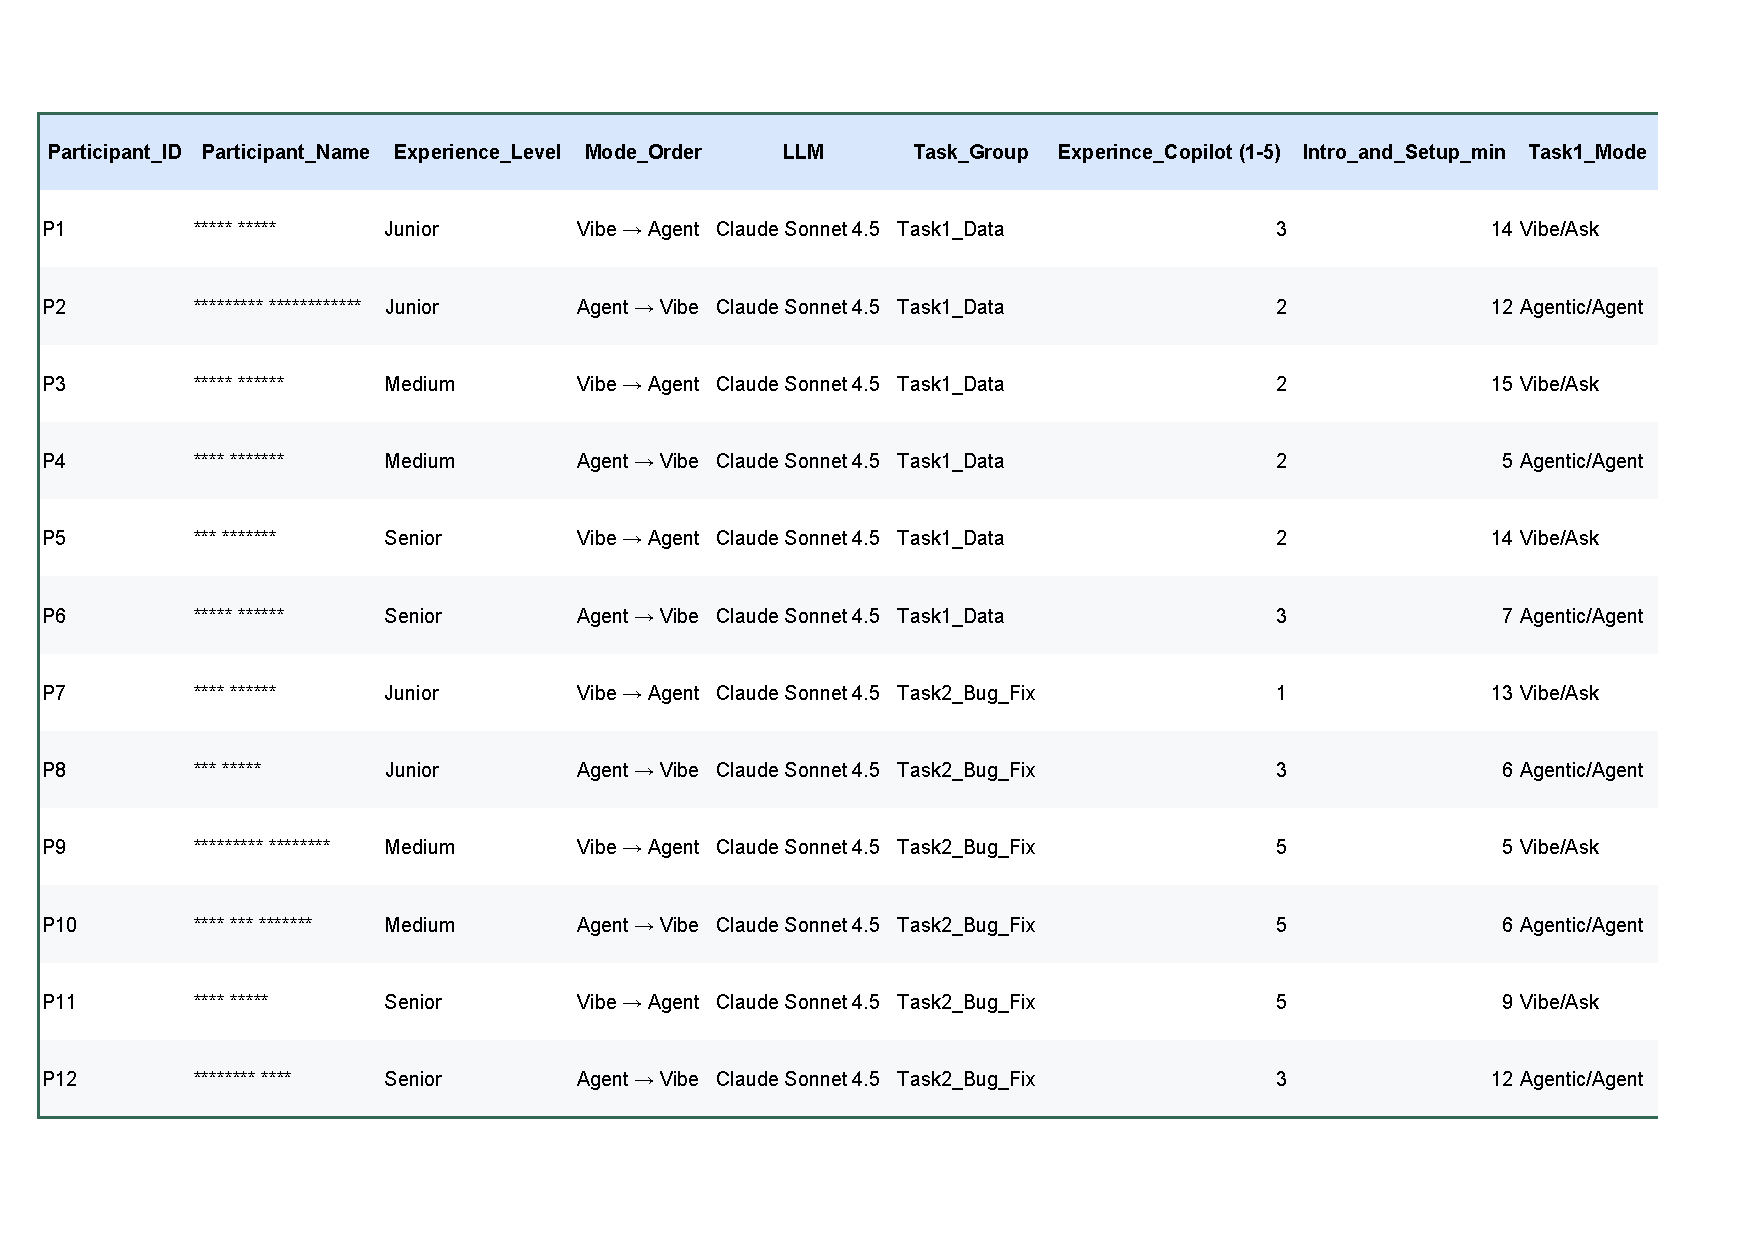
\includepdf[
  pages=-,
  fitpaper=true,
  scale=1,
  offset=0 0,
  pagecommand={\thispagestyle{plain}}
]{figures/master_thesis.pdf}
\end{landscape}



\end{appendices}


\end{document}
